% !Mode:: "TeX:UTF-8"
\documentclass[master,openright,twoside,color]{buaathesis}
\usepackage{booktabs}
\usepackage{graphicx}
\usepackage[ruled]{algorithm2e} % For algorithms
\renewcommand{\algorithmcfname}{ALGORITHM}
\begin{document}

% 用户信息
% !Mode:: "TeX:UTF-8"

% 学院中英文名,中文不需要“学院”二字
% 院系英文名可从以下导航页面进入各个学院的主页查看
% http://www.buaa.edu.cn/xyykc/index.htm
\school
{计算机}{School of Computer Science \& Engineering}

% 专业中英文名
\major
{计算机应用技术}{Computer Science and Technology}

% 论文中英文标题
\thesistitle
{基于神经网络的高性能语言建模技术研究}
{}
{Nerual Network Based Highly Efficient Language Modeling}
{}

% 作者中英文名
\thesisauthor
{姜楠}{Jiang Nan}

% 导师中英文名
\teacher
{荣文戈}{Rong Wenge}
% 副导师中英文名
% 注:慎用‘副导师’,见北航研究生毕业论文规范
%\subteacher{副导师}{subteacher}

% 中图分类号,可在 http://www.ztflh.com/ 查询
\category{TP391}

% 本科生为毕设开始时间;研究生为学习开始时间
\thesisbegin{2015}{09}{01}

% 本科生为毕设结束时间;研究生为学习结束时间
\thesisend{2018}{}{}

% 毕设答辩时间
\defense{2018}{}{}

% 中文摘要关键字
\ckeyword{层次概率,神经语言模型,递归神经网络,自然语言处理}

% 英文摘要关键字
\ekeyword{Hierarchical Softmax, Neural Language Model, Recurrent Neural Network, Natural Language Processing.}
% !Mode:: "TeX:UTF-8"

% 研究方向
\direction{自然语言处理}

% 导师职称中英文
\teacherdegree{副教授}{Associate Prof.}
% 副导师职称中英文
% 注:慎用‘副导师’,见北航研究生毕业论文规范
%\subteacherdegree{讲师}{Teacher}

% 保密等级,注:非保密论文时不需要此项
%保密论文请更改‘buaathesis.cls’里相应代码
%\mibao{机密}

%申请学位级别
\applydegree{工学硕士}

% 论文编号,由10006+学号组成
\thesisID{10006SY1506330}

% 论文提交时间
\commit{2018}{}

% 学位授予日期
\award{2018}{}{}


% 中英封面、提名页、授权书
\maketitle
% 前言页眉页脚样式
\pagestyle{frontmatter}
% 摘要
\begin{cabstract}
最近在自然语言处理中,已经提出了基于神经网络结构的变体,并成功地应用于神经语言模型和神经声学模型。这些神经模型可以通过学习来自大规模语料库的参数来利用知识,而对于真实世界的挑战来说,它们是非常缓慢的,因为它们在训练和推理期间预测来自大词汇量的候选者。作为基于抽样的近似的替代,我们探索历史提出的基于树和基于类的分层softmax方法。在这项研究中,为了减少计算时间,并使其与现代图形处理单元兼容,我们引入了一系列高效和有效的方法,并将我们的贡献归类为:a)首先,我们改进它们的结构组成并引入一个compact基于树和基于类的相应的分层softmax方法的损失函数; b)其次,我们讨论几种基于ngram的句法和语义聚类算法对香草层级softmax的影响,因为它们对聚类方法敏感; c)第三,我们讨论了可能的分层softmax变体的推理算法,保证模型可以在不同情况下获取可能的预测结果。最后,我们用标准基准数据集,即WikiText-2,WikiText-103和十亿字数据集对语言建模任务进行了我们的实验。与其他传统的优化方法相比,还实现了几个内在的评估标准:字错误率和困惑度的改进。
\end{cabstract}

\begin{eabstract}
Recently in natural language processing, variants of neural networks based architecture have been proposed, and successfully applied to neural language models and neural acoustic models. These neural models can leverage knowledge by learning parameters from massive corpora, while they are extremely slow for the real world challenge as they predict candidates from a large vocabulary during training and inference. As an alternative to sampling-based approximation, we explore the historical proposed tree-based and class-based hierarchical softmax methods. In this research, aiming at reducing its computational time as well as making them compatible with modern graphics processing units, we introduce a series of efficient and effective approaches and categorise our contributions as: a) Firstly, we reform their structural composition and introduce a compact tree-based and class-based loss function for the corresponding hierarchical softmax methods; b) Secondly, we discuss the impact of several ngram-based, syntactic and semantic clustering algorithms for the vanilla hierarchical softmax as they are sensitive to clustering methods; c) Thirdly, we discuss possible inference algorithms for the hierarchical softmax variants, assuring the model can fetch presumable predictions under different circumstances. Finally, Our experiments were carried out on language modelling tasks with standard benchmarks datasets, i.e., WikiText-2, WikiText-103 and One Billion Word datasets. Consist improvement with several intrinsic evaluation criterions: word error rate and perplexity, were also achieved over other conventional optimisation methods.
\end{eabstract}
% 目录、插图目录、表格目录
\tableofcontents
\listoffigures
\listoftables
% 符号表
%\include{data/master/denotation}

% 正文页码样式
\mainmatter
% 正文页眉页脚样式
\pagestyle{mainmatter}

\chapter{绪论}
\section{课题来源与意义}
近几年来,随着互联网(Internet)的兴起和发展,互联网上积累的数据呈现急剧膨胀的态势。根据国际数据信息公司\footnote{https://www.idc.com/}(International Data Corporation, IDC)的统计和预测,2018~年全球网络数据量已经达到~1.8~ZB,预计到~2025~年,全球网站数据累积总量还将增长约~50~倍。
随着这类文本、视频、图像无标注的数据(Unlabeled Data)的大量涌现,如何利用现有的机器学习算法(Machine Learning),从这类已存在的大量的无标注数据中学习内在规律和知识以提取出有用的信息,已经变成了一个重要的挑战\upcite{王建翔2017面向可读性评估的词向量技术研究及实现}。
自从2006 年,以~Geoffrey Hinton~为代表的学者们提出的深度学习(Deep Learning, DL)理念~\upcite{hinton2006reducing}以来,这一新的思路为解决如何利用爆炸的数据量,以提取有效知识带来了新的前景。
在这之后的发展中,基于神经网络(Neural Network,NN)的表示学习技术(Representation Learning)开始快速拓展到各个相关研究领域中去。
尤其在图像分类(Image Classification)、语音自动识别(Automatic Speech Recognition,ASR)~\upcite{DBLP:journals/taslp/WangW16}和神经机器翻译(Neural Machine Translation,NMT)~\upcite{bahdanau2014neural}领域的多个任务上,基于深度模型的方法,在精确度和效率上远远超过了基于特征提取(Feature Extraction)的传统方法。

随着应用领域的拓展,深度学习技术逐渐在自然语言处理中(Natural Language Processing, NLP)得到广泛应用。 例如,蒙特利尔大学教授 Yousha Bengio 提出用神经网络来训练语言模型(Language Model,LM),并对模型中的各个结构细节进行了相关探索\upcite{DBLP:conf/nips/BengioDV00}。因为输入的维度是固定的N个单词的词向量,而不是动态长度,所以该方法不能有效处理单词的长距离单词依赖问题。
针对这个问题,在后续的工作中,由其学生~Tomas Mikolov~提出了采用循环神经网络(Recurrent Neural Network, RNN)\upcite{DBLP:journals/cogsci/Elman90}对上下文信息作为建模策略的方法,并逐步将该理论进行了拓展和简化\upcite{DBLP:conf/interspeech/MikolovKBCK10}。
循环神经网络主要特点是能够记忆该单词之前的所有出现过的单词的信息,即所谓的全局上下文信息(Global Context),用来预测下一个单词出现的对数概率分布。
因为RNN模型在训练过程中学习到了单词的前面出现的所有词,所以句子的长距离依赖关系(Long Term Dependency)可以被学习到,所以该方法在建模理论上克服了最初的神经网络语言模型的无法利用语句长距离上下文依赖的缺点。
另外,在模型训练的过程中,语义相似的单词被映射到的某低维子空间中,也满足了单词的语义相似(Semantic Similarity)的要求。相比统计语言模型(Statistical Language Model)领域中的N-gram模型,他不需要平滑技术(Smoothing Technology)来对文本中出现次数少的单词做处理。
到目前为止,RNN~模型已经演变出各种结构,应用在非常多的文本任务上面,并且都能取得了较为满意的结果。

由于RNN网络的计算时间与句子的平均长度正相关,所以基于~RNN~建模的算法计算时间都很大,需要更长的时间收敛。同时,我们需要看到最简单的RNN模型所使用的参数数量是NPLM模型的两倍多,这也意味着RNN模型需要占用更大的内存空间,消耗了更多的计算资源,导致其无法广泛应用到现实场景中去。
在文献~\cite{DBLP:conf/icassp/MikolovKBCK11}~中,Tomas Mikolov 提出了多种优化策略来消除该模型的各种缺点,例如:缩短模型求导步数、对词表(Vocabulary)做分解~\upcite{DBLP:journals/coling/BrownPdLM92}等策略,这些计算策略能保证模型的计算精度,同时极大提高了RNN网络的运算效率。

\section{国内外研究现状}
语言模型可以用来估算一段文序列组合的可能性,该模型在机器翻译(Machine Translation)、语音识别(Speech Recognition)等任务上都有着极为重要的作用。考虑到语言模型的漫长的发展历史,我们可以划分为两个主要阶段:统计语言模型(Statistical Language Model)和神经网络语言模型(Neural Language Model)。
其中,统计模型指代的是~N-gram~语言模型,而随着深度学习的爆发,各种神经网络语言模型变体逐渐发展并占据了主导地位。我们接下来会对这两个演化阶段所涉及的算法一一介绍。

\subsection{N-gram 语言模型}
首先介绍传统的~N-gram~语言模型,该算法属于典型的基于稀疏表示(Sparse Representation)的语言模型,因为一个单词表示方式是独热表示(One-Hot Representation)。该传统模型的意义不仅是提供了一种文本建模策略,而且定义了如何评价语言模型的好坏,并且定义了语言模型所涉及的相关拓展方向。

接下来给出~N-gram~统计语言模型的形式化定义。假设给定一个长度为$m$ 的单词字符串,$w_1$ 到$w_m$ 依次表示这段文本中的各个单词,我们需要求解一个概率分布$p(w_1,\cdots,w_m)$,以表示该字符串存在或者出现的可能性。在求解过程中,我们通常使用链式法则(Chain Rules),将计算整个序列概率问题分解成如下形式:
\begin{equation}
\setlength{\abovedisplayskip}{6pt}
\setlength{\belowdisplayskip}{6pt}
\label{equ:lm}
p(w_1,\cdots,w_m) =p(w_1)\prod_{t=1}^{m}p(w_t|w_1,\cdots,w_{t-1})
\end{equation}
在实际求解过程中,如果文本的长度较长,公式~(\ref{equ:lm})~中右部~$p(w_m | w_1,w_2,\cdots,w_{m-1}) $ 的估计误差会很大。因此,提出了~N~元模型(N-gram model),它能简化了实际问题的复杂度,最早被用来估算条件概率。需要注意的是,单词距离大于$n$单词会被直接忽略,该模型可以写成如下形式:
\begin{equation}
\setlength{\abovedisplayskip}{6pt}
\setlength{\belowdisplayskip}{6pt}
\label{equ:approx}
p(w_i | w_1,w_2,\cdots,w_{t-1})  \approx p(w_i | w_{t-(n-1)},\cdots,w_{t-1})
\end{equation}
假若~$n=1$~,此时称其为一元模型(Uni-gram model),公式~(\ref{equ:approx})~将会退化成~$p(w_i),i\in [1,n-1]$.此时,整个句子的概率计算公式为:~$p(w_1,w_2,\cdots,w_m) = p(w_1)p(w_2) \cdots p(w_m)$。
从这个退化的公式中,可以得知:在一元模型中,整个文本的概率是出现的各个单词的词频概率的乘积,它直接丢失了文本词组之间的顺序信息。当~$n = 2$~时,称为二元模型(Bi-gram model),公式~(\ref{equ:approx})~将会退化为 $p(w_t|w_{t-1})$。除此之外,还有 $n=3$ 时的三元模型(Tri-gram model),使用$p(w_t |w_{t-2},w_{t-1})$ 作为近似概率分布。当~$n>1$~的模型均可以保留一定的词序信息。

传统方法采用单词或者n元组的词频来作为n元组的概率计算方法,该方法简单有效能满足线上负载的计算需求。但是随着n的增大,模型的参数呈现指数爆炸式增长、概率计算复杂度也相应上升。目前谷歌有在线存储的最大的~9~元模型(Google N-gram Viewer)\footnote{https://books.google.com/ngrams},这已经是目前计算机系统存储,数据访问的极限了。


神经网络的建模思路源自于~N-gram~模型,它主要解决的问题是如何对文本的上下文信息利用先用的模型进行建模。历史上的模型,我们可以主要划分为:传统前向传递神经网络(Feed Forward Neural Network, FFNN)、循环神经网络(Recurrent Neural Network, RNN)以及双线性模型(Bilinear Model)这三种建模方案。 以下我们将一一探讨。


\subsection{前馈神经网络语言模型}
由于神经网络对参数进行高度共享,因此对低频词具有天然的平滑能力。这里所指的神经网络语言模型(Neural Probabilistic Language Model, NPLM) ,最早由Bengio等人在2001年提出\upcite{DBLP:conf/nips/BengioDV00}, 近年来一些学者开始展开这方面的研究,并取得一系列成果,如~\cite{DBLP:conf/acl/BaroniDK14,DBLP:journals/sigkdd/BellK07,DBLP:journals/pami/BengioCV13,DBLP:journals/tnn/BengioSF94}~。 但总体而言, 对NPLM的研究还处在起步阶段。具体而言,NPLM通过一个多层感知网络(Multi-Layer Perceptron, MLP)来计算公式~(\ref{equ:approx})~中概率。
\begin{figure}
  \centering
  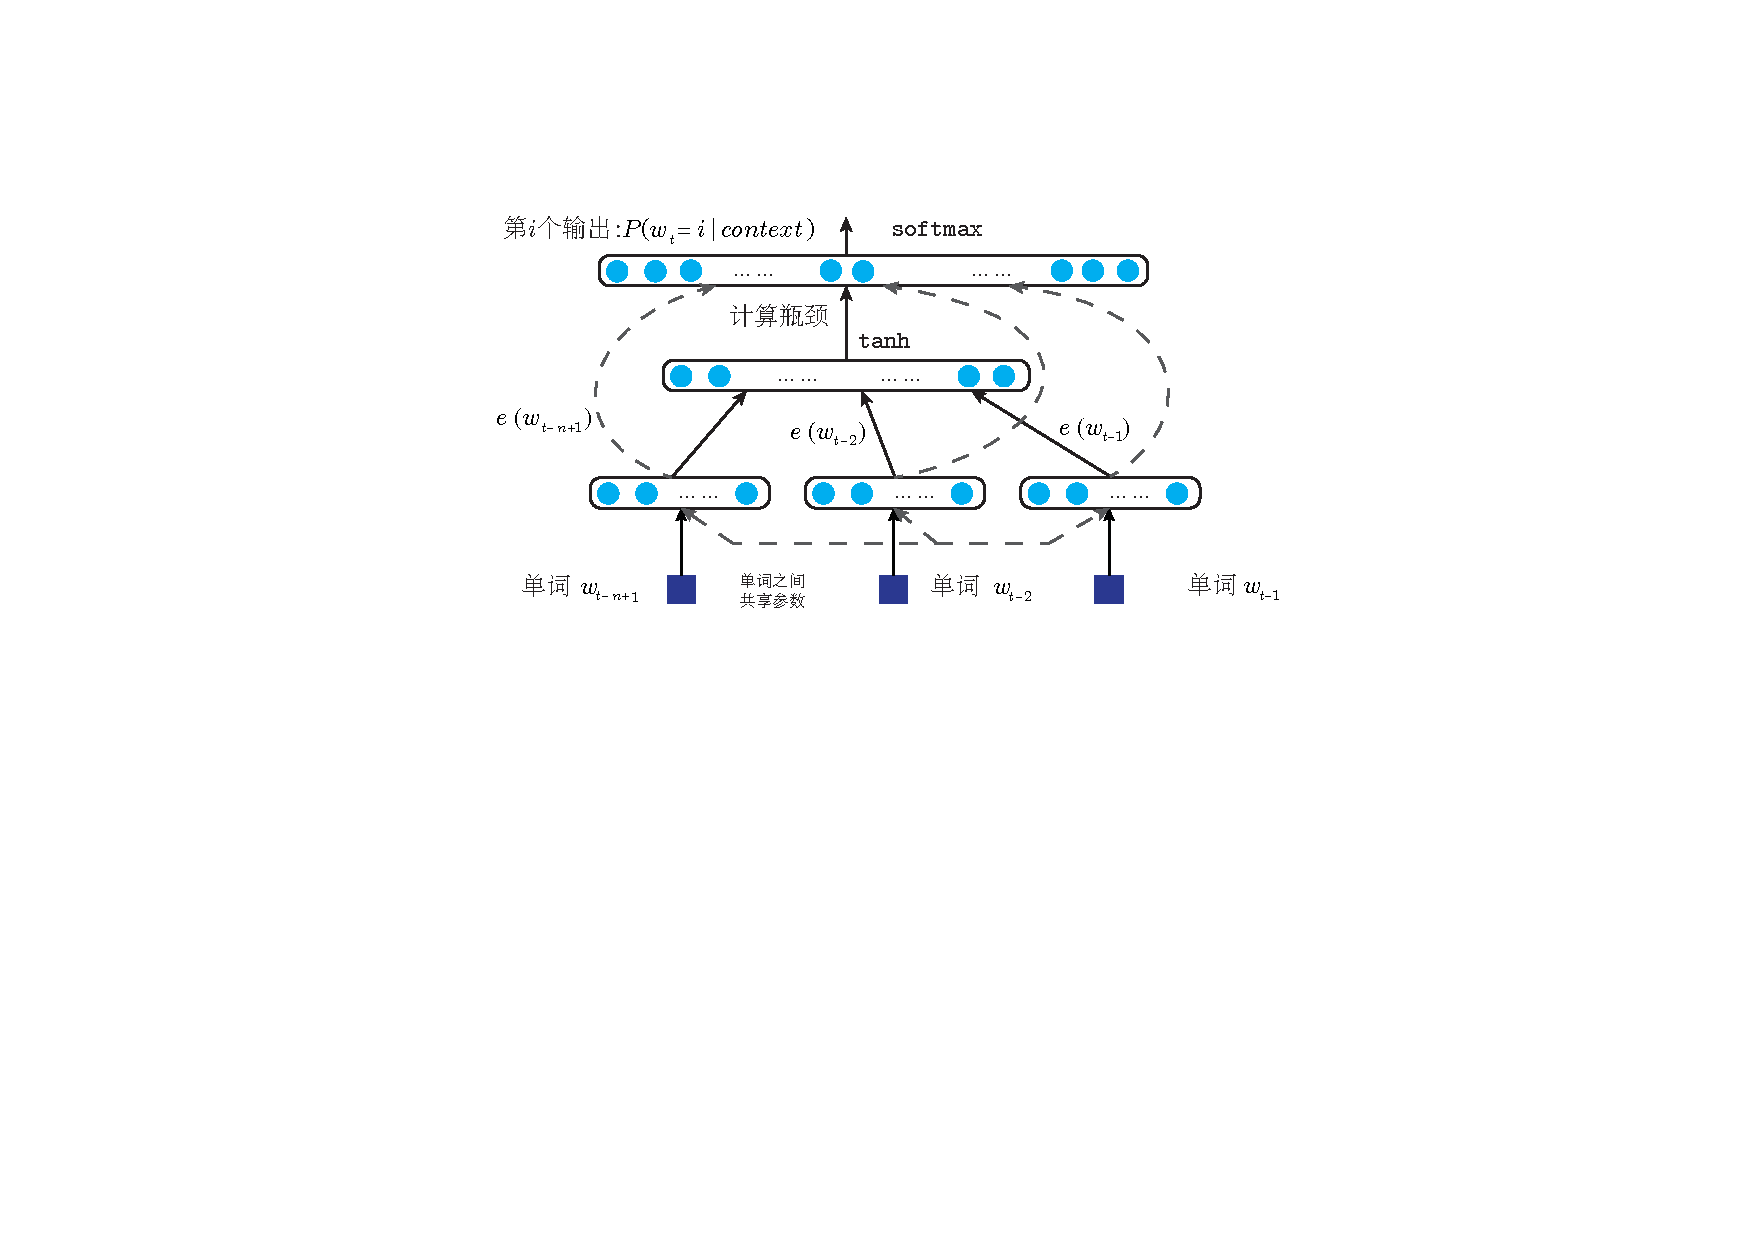
\includegraphics[width=.85\linewidth]{./figures/nplm.pdf}
  \caption{前馈神经网络语言模型}\label{fig:nplm}
\end{figure}

图~\ref{fig:nplm} 给出一个典型的采用三层前馈神经网络结构 NPLM 语言模型。其中输入层用于表征前$n$个单词的高维分布;隐藏层,表征单词的上下文信息,最后一层是输出预测层,预测下一时刻的可能出现的单词概率分布。为了解决数据稀疏问题,Bengio~等人提出拼接(Concatenation)各词的词向量作为输入,如下所示:
\begin{equation}\label{equ:we}
  x = [e(w_{i-(n-1)}), \cdots , e(w_{i-2}), e{(w_{i-1})}]
\end{equation}
模型的隐藏层$h$ 和输出层$y$可以依照下面的公式计算获得:
\begin{equation}\label{equ:nplm}
\setlength{\abovedisplayskip}{6pt}
\setlength{\belowdisplayskip}{6pt}
\begin{split}
h =& \tanh(Hx+b) \\
y =&Wx + Uh +b'
\end{split}
\end{equation}
其中参数矩阵~$H,W,U$~指代层与层之间的权重\upcite{赵林2007一种新的基于结构的神经网络规则抽取方法},参数向量~$b,b'$~均为模型中的偏置项(Bias)。如果存在$W$,那么模型能直接学习一个线性模型,需要训练的时间减少;如果不存在$W$,模型学习到非线性的网络模型,具有更好的泛化性(Generalization)。因此在后续工作中,很少有使用输入层到输出层直连边的工作,下文我们也直接忽略这一种直连的操作。假设不考虑$W$ 矩阵,整个模型计算量最大的运算,就是从隐藏层到输出层的矩阵运算$Uh$,后续的模型均有对这一矩阵乘法计算做优化。

\subsection{对数双线性语言模型}
2007 年,Mnih 和 Hinton 在神经网络语言模型(NNLM)的基础上提出了对数双线性语言模型(Log-Bilinear Language Model, LBL)~\upcite{DBLP:conf/icml/MnihH07}。LBL~模型与~NNLM~模型的区别正如它们的名字所示,其中~LBL~的模型结构是一个对数双线性结构;~NNLM~的结构不包含双线性结构,仅仅是简单的前馈网络。具体来讲,LBL 模型的代价函数为:
\begin{equation}
\setlength{\abovedisplayskip}{6pt}
\setlength{\belowdisplayskip}{6pt}
\label{equ:lbl}
\begin{split}
   &\hat r=\sum_{i=1}^{n-1}{U_i e({w_i})}, \\
   &p(w_n=w|w_{1:n-1})=\frac{\exp(\hat r^\top e(w))}{\sum_j{\exp(\hat r^\top e(w_j))}}
\end{split}
\end{equation}
其中 $\hat r$ 代表了语言模型的上下文信息,$U_i$ 指代的是对应单词的权重向量。然后基于上下文信息表示 $\hat r$ 和下一个单词的目标词汇表中所有单词 $e(w),w\in \mathcal{V}$ 的表示之间的相似度来计算下一个单词的可能的概率分布。

公式~(\ref{equ:lbl})~所描述LBL模型的代价函数与公式~(\ref{equ:nplm})~所描述~NNLM~模型的代价函数的主要区别有:1) LBL 模型中,没有非线性的激活函数$\tanh$,而由于NNLM 是非线性的神经网络结构,激活函数必不可少;2) LBL 模型中,只有一份词向量$e$,也就是说,无论一个词是作为上下文,还是作为目标词,使用的是同一份词向量。其中第二点(只有一份词向量),只在原版的LBL 模型中存在,后续的改进工作均不包含这一特点。

后来,Mnih~等人以~LBL~模型为基础,并对其所存在缺点做了一系列改进工作。其中最重要的模型有两个:逆向量语言模型(inverse vector LBL,ivLBL)~\upcite{DBLP:conf/nips/MnihK13}和层次对数双线性语言模型(Hierarchical LBL,HLBL)~\upcite{DBLP:conf/icml/MnihT12}。

\subsection{循环神经网络语言模型}
对于循环神经网络来说,它能直接对序列概率~$p(w_t | w_1,w_2,\cdots,w_{t-1})$~进行建模,而不使用公式~(\ref{equ:approx})~对其进行简化~\upcite{mikolov2012statistical,DBLP:conf/interspeech/MikolovKBCK10} 。RNNLM 模型结构如图~\ref{fig:rnnlm}~所示,它的核心方法在于其隐藏层的计算公式:
\begin{equation}
\setlength{\abovedisplayskip}{6pt}
\setlength{\belowdisplayskip}{6pt}
\label{equ:rnn}
  h_t \leftarrow  \phi(e(w_t) + U h_{t-1} +b),
\end{equation}
其中 $\phi$ 为非线性激活函数。在上述公式中,$h_t$ 表示文本中第 $t$ 个词 $w_t$ 所对应的隐藏层,该隐藏层由词向量 $e(w_t)$ 以及上一个步的隐藏层输出 $h_{t -1}$ 计算得到。隐藏层的初始状态为$h_0$,随着模型逐个读入单词:$w_1,w_2,\cdots$, 隐藏层根据公式~(\ref{equ:rnn})~被计算出来并被输出:$h_1,h_2,\cdots$ 。通过这种自身迭代更新方式,囊括了此单词前所有上文的信息,相比NPLM模型,RNNLM 理论上能学习到更丰富、更长距离的知识,也有更大的潜力达到更好的效果。最后,RNNLM 模型的输出层与NPLM 模型的输出层都采用softmax算法,两者是一致的。

\begin{figure}
  \centering
  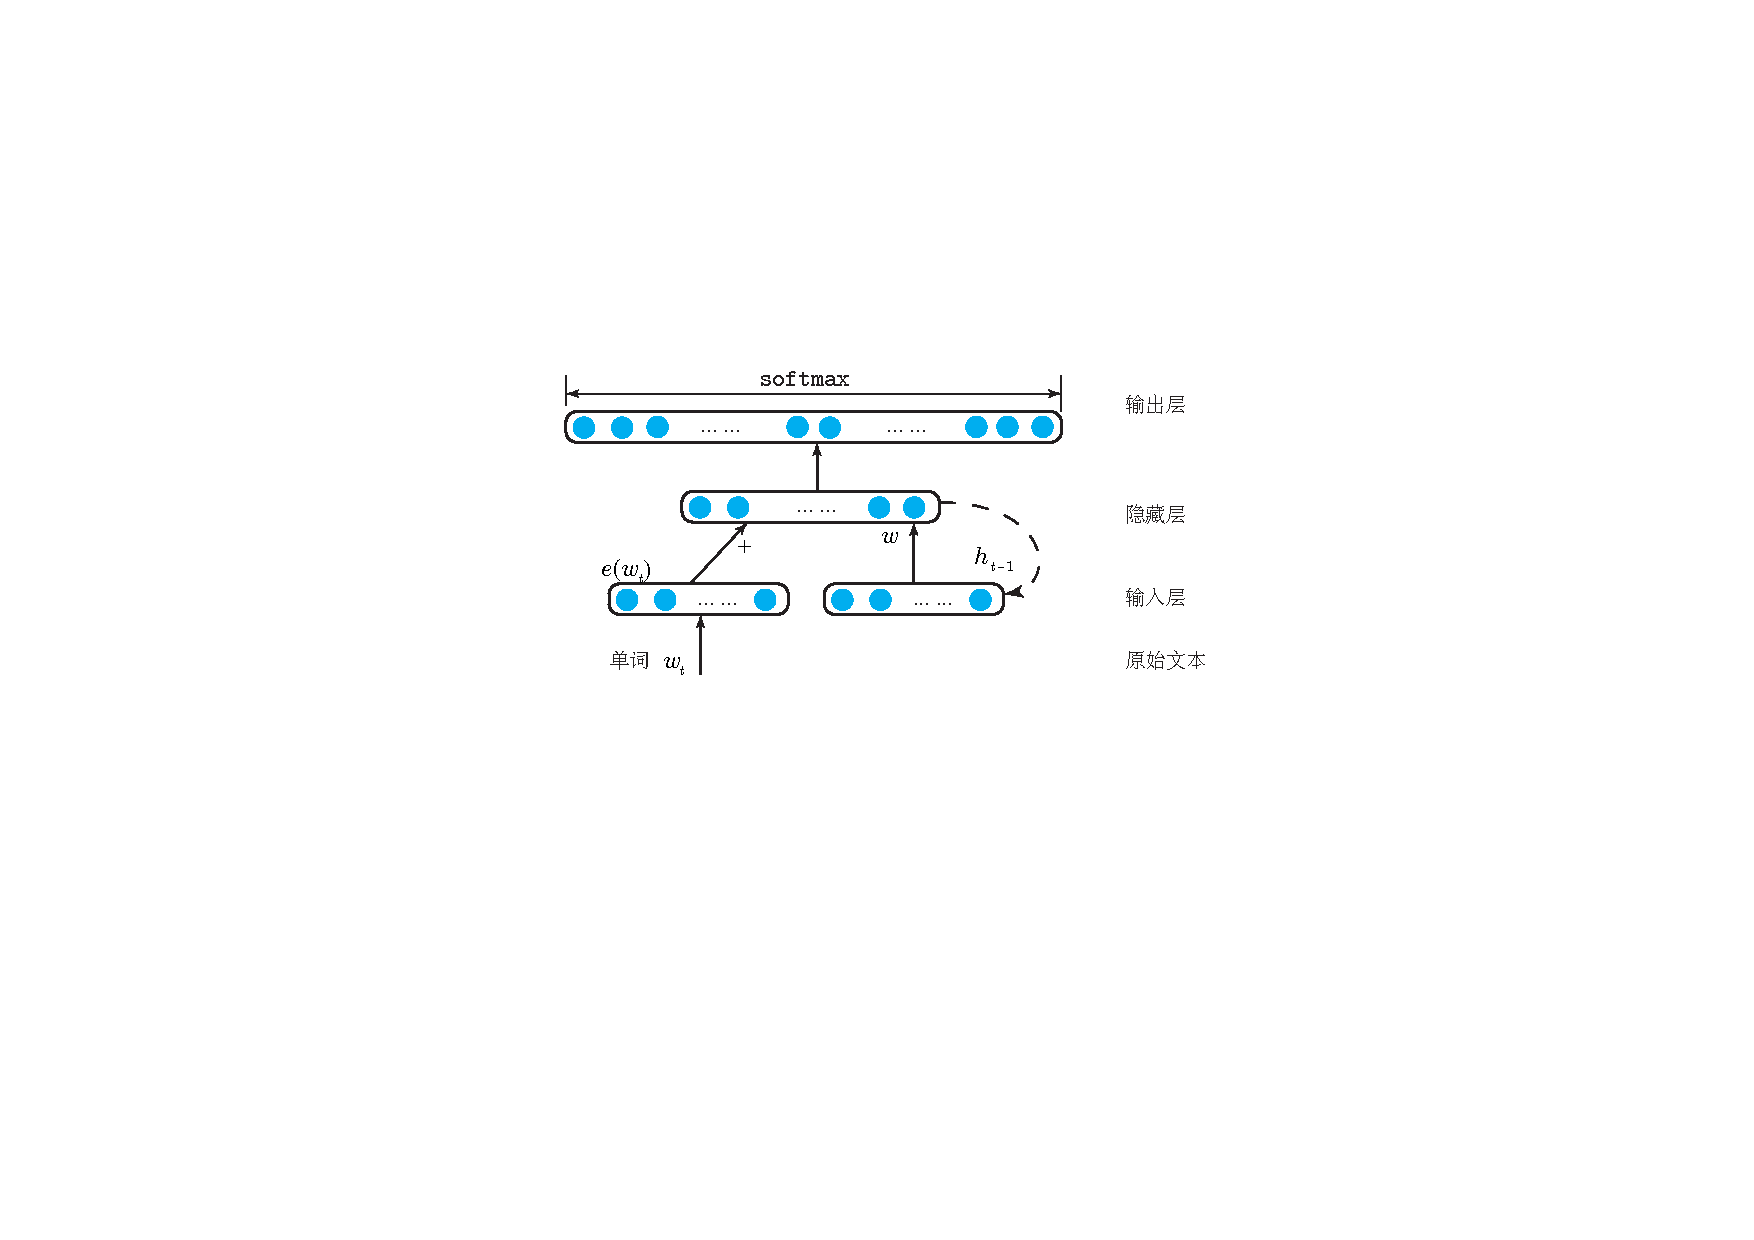
\includegraphics[width=.8\linewidth]{./figures/rnnlm.pdf}
  \caption{循环神经网络语言模型结构图}\label{fig:rnnlm}
\end{figure}


除了介绍的两种经典的建模方法,最近研究者提出可以使用带有门限机制(Gating)的RNN来防止模型的长距离依赖问题,例如长短记忆网络(Long Short-Term Memory, LSTM), 门限记忆节点(Gated Recurrent Unit, GRU)和其他网络。


\section{论文研究内容}
在历史文献当中,源词和目标词分别被称为模型的输入和输出。源词通常可以用分布式表示(Distributed Representation)来表示,称为输入词嵌入(Word Embedding),可以使用基于外部语料库的连续词袋模型(CBoW)或跳跃单词模型(Skipgram)模型来训练。而这两个模型来源于语言模型任务,并且为了在特征空间中产生可能的嵌入分布而被大大简化。另外,输出字通常表示为字索引(Indexing)或~$1-K$~编码,并且可以与softmax概率函数直接关联。

语言模型的大词表问题是目前理论应用到实际过程中必须要克服的问题,我们当然可以通过配置高性能服务器来暂时延缓该问题的后果。但是一旦应用到大数据集上,即使是目前最好的中央处理器(CPU)或者图形处理器通用计算(GPGPU),仍然需要一个多月时间才能训练完善。因此,在保证原有模型的准确率和精度的前提下,如何提高模型的训练速度是我们主要讨论和研究的内容。为此我们讨论了两个不同的内容:上下文信息建模效率和精度对比和大词表问题的优化和研究。

针对上下文信息建模手段,目前主要采用的方案有以下几种:一种是采用子词(Subword-level)或者字符级别的词(Character-level)来直接缩小词表大小;一种是通过采样技术(Sampling-based Approximation)来减少必要的训练时间;一种是通过基于分类的多元分类(class-based Hierarchical Softmax, cHSM)来加速模型和采用基于树模型的多层二元分类模型(tree-based Hierarchical Softmax, tHSM)。同时,我们还需要针对CPU 和GPGPU设备分别进行探讨。因为传统的线性运算模型在流行的GPGPU并行运算方案中并不适用,所有需要结合不同的运算设备分别讨论可行的方案。

在本节中,我们将这个目标词表示扩展到一个分层的形式,使它们适配基于类和基于树的分层概率计算。首先,我们提出了一个在分层结构上建模参数的字编码方案。因此,考虑到~GPGPU~上的并行吞吐性能,我们推导出紧凑的代价函数及其梯度。同时,类或树上的单词分布对其性能有很大的影响,应该在训练阶段之前定义,这些动态交换算法在训练过程中改变了单词群或子树结构在这个研究中。我们采用了几个分层聚类和词汇分割策略,用统计,句法和语义知识来初始化其结构,以达到一个稳定和可以预期的性能。而且,在推理过程中,不同于传统的softmax情况,得到最好的候选者自然是可行的,层次推理不能直接用 softmax 方法来实现。我们讨论基于树和基于类的搜索策略的两种不同的推理情况:1)打分:输出给定序列的概率;2)排序   :在给定的上下文中获取得分最高的一个候选单词。
\section{论文的组织结构}
\textbf{第一章:}``绪论'',主要介绍了本论文的研究背景和意义,另外简要说明了语言模型的发展历史以及本文的主要工作,并对本文的组织架构进行了说明。

\textbf{第二章:}``相关技术介绍'',对历史上的各个学术流派在语言模型的任务上相关工作进行了介绍。

\textbf{第三章:}``并行树状概率模型'',介绍了基于二叉树的层次概率模型,并比较了传统树状模型的差一点。同时还研究了在推理测试阶段,二叉树层次概率模型能应用的策略,以保证实际测试结果性能和效率。


\textbf{第四章:}``并行分类层次概率模型'',介绍基于分类的层次概率模型,并分析了词表非均匀划分所产生的后果,进而探讨了类别不均匀问题所带来的影响以及相关解决策略。最后探讨了在测试阶段,语言模型的任务需求和分类层次概率模型相应的解决算法。

\textbf{第五章:}``语言模型实验及实验结果分析'',实证研究了本论文提出的并行层次概率模型的实际效果,并和其他算法在各个指标维度上进行了比较和分析。

最后结论部分,总结了全论文的贡献和工作,并提出了未来的工作方向,同时撰写了结束语。







\chapter{相关技术介绍}

\section{已经完成的工作}
基于神经网络的分布表示一般称为词向量、词嵌入(Word Embedding)或分布式表示(Distributed Representation)~\upcite{DBLP:conf/nips/MikolovSCCD13}。神经网络词向量表示技术通过神经网络技术对上下文,以及上下文与目标词之间的关系进行建模。由于神经网络较为灵活,这类方法的最大优势在于可以表示复杂的上下文。在前面基于矩阵的分布表示方法中,最常用的上下文是词。如果使用包含词序信息的n-gram 作为上下文,当n 增加时,n-gram 的总数会呈指数级增长,此时会遇到维数灾难问题。而神经网络在表示n-gram 时,可以通过一些组合方式对n 个词进行组合,参数个数仅以线性速度增长。有了这一优势,神经网络模型可以对更复杂的上下文进行建模,在词向量中包含更丰富的语义信息。神经网络模型主要包括: 传统前向传递神经网络(Feed Forward Neural Network, FFNN)、循环神经网络(Recurrent Neural Network, RNN)建模方案。

另外针对大词表问题,主要可以分为以下两种策略:基于类别的多元分类模型(class-based hierarchical softmax, cHSM)和基于二叉树的二元分类模型(class-based hierarchical softmax,tHSM),我们分别在下面详细讨论和介绍。


\subsection{完成的工作内容: 上下文信息建模}


\subsection{完成的工作内容: 大词表问题的优化}
传统的多元分类模型(Softmax):
\begin{equation}
\label{eq:softmax}
\begin{split}
%p(w_i|h)=&\frac{\exp(h^\top v_{w_i})}{\sum_{w_j\in \mathcal{V}}{\exp(h^\top v_{w_j} )}} \\
\log p(w_i|h) &= \theta^w_i h-\log \sum_{w_j\in \mathcal{V}}{\exp(\theta^w_j h)}\\
%\frac{\partial p(w_i|h)}{\partial v_{w_j}}=&p(w_j|h)(\delta_{ij}-p(w_i|h))h^\top\\
\nabla_{\theta^w_j}{\log p(w_i|h)}&= (\delta_{ij}-p(w_i|h))h
\end{split}
\end{equation}
其中 \textit{Kronecker delta} 函数的定义为: $\delta_{ij} = 1$ 如果 $i = j$。 $h$ 是隐藏层输出的向量,并且 $\theta^w$ 是目标端的词向量 $w$~\upcite{duda2012pattern}.

其中由于分母是正则项,一旦词表扩大,每次迭代更新都需要计算这一项,是主要的问题所在,所以本课题拟在主要解决该问题所导致的计算费时的问题,在保证计算精度不下降的情况下,提高模型的训练速度。 目前主要的算法分为以下三类: 单词拆分算法、采样估计模型和层次分解模型。


\subsubsection{单词拆分算法}
最直接的算法就是我们放弃使用大词表,转而保留一个较小的词表来保证训练的内存占用和计算效率。那么针对过多的词表外的单词(Out-Of-Vocabulary,OOV),我们可以使用传统的N-gram语言模型来估算其可能的概率分布。这样做一方面保证神经网络模型可以在有限时间内训练完,同时保证模型的最后的测试结果不会很差~\upcite{DBLP:journals/csl/Schwenk07}。当我们的词表继续增大的时候,我们会发现训练样本中存在过多的$\langle$unk$\rangle$ 字符,这样使得神经网络的模型训练非常苦难导致效果变得不可接受,所以这种方案只是一定程度上缓解了大词表问题,但是也是一种有效的尝试方案。

\begin{figure}
  \centering
\includegraphics[width=0.6\linewidth]{./figures/subword.png}
\caption{词到子词划分样例.单词背划分成前缀和后缀,其中$+$代表是单词的前缀同时$\langle /w \rangle$是单词的后缀。}\label{fig:subword}
\end{figure}
除了上述方案,目前采用的方案是将单词按照字符级别来划分,可以将一个单词按照字符统计规律划分成任意多个子词。其中二元对编码(byte-pair-encoding,BPE)能将一个单词划分成两部分:前缀(Prefix)和后缀(Suffix)~\upcite{DBLP:conf/icassp/Tucker0P94, DBLP:conf/acl/SennrichHB16a,Gage:1994:NAD:177910.177914},如图.~\ref{fig:subword} 所示。由于划分规则是从训练数据中学习到的,我们可以指定需要缩减的词表大小,该算法的动态适应性很强,目前主流的机器翻译模型都采用这个方案~\upcite{DBLP:journals/corr/JozefowiczVSSW16}。尽管如此,我们仍然需要看到它这样的解构操作依然带来了一定的损失,因为句子的长度增倍了,对RNN的长距离关系学习能力提出了更高的挑战~\upcite{DBLP:conf/aaai/KimJSR16}。

\subsubsection{采样估计模型}
目前采用的采样算法主要是针对概率规约那一项进行概率估计,其中著名的算法有:重要性采样(Importance Sampling)~\upcite{DBLP:journals/tnn/BengioS08},噪声差分估计(Noise Contrastive Estimation, NCE)~\upcite{DBLP:conf/icml/MnihT12}和Blackout 采样算法~\upcite{DBLP:journals/iclr/JiVSAD15}。第一种算法在实验中被证明模型无法收敛,目前主要使用的后面两种算法。

对于噪声差分估计算法来说,模型需要学习将正确的单词 $w_0$ 与随机生成的单词 $\{w_1\cdots w_k\}$做一个二元分类。 其中 $w_0$ 训练样本中真正的下一个单词, $\{w_1\cdots w_k\}$ 是采用先验分布  $q(w)$产生的随机噪声单词. 正例归一化后的概率和所有负例联合概率的公式可以写成:
\begin{equation}\label{equ:nce}
\begin{split}
  \tilde{p}(y=1|h)=&\frac{\exp( \theta^w_0 h)}{ \exp( \theta^w_0 h)+k *q(w_0)}\\
  \tilde{p}(y=0|h)=&\prod_{i=1}^{k}\frac{k *q(w_i)}{\exp( \theta^w_i h)+k *q(w_i)}\\
\end{split}
\end{equation}
需要注意的是 $\tilde{p}(y=0|h)$ 需要对 $k$ 个噪声样本做加法运算而不是对整个词表单词进行的。 这样的话该算法的计算机复杂度就是$\mathcal{O}(k)$,和整个词表的大小无关了。除此之外,最近提出的Blackout采样算法针对噪声概率归一化的时候与当前上下文的相关,对NCE算法进行了进一步修改~\upcite{DBLP:journals/iclr/JiVSAD15}。

\subsection{层次分解模型}
目前主要的策略分为: 基于类别的多元分类模型(class-based hierarchical softmax, cHSM)和基于二叉树的二元分类模型(class-based hierarchical softmax, tHSM)。图.~\ref{fig:case_hsm}展示了第一种算法的示例,图.~\ref{fig:tree_hsm}展示了第二种算法的示例。
\begin{figure}
  \centering
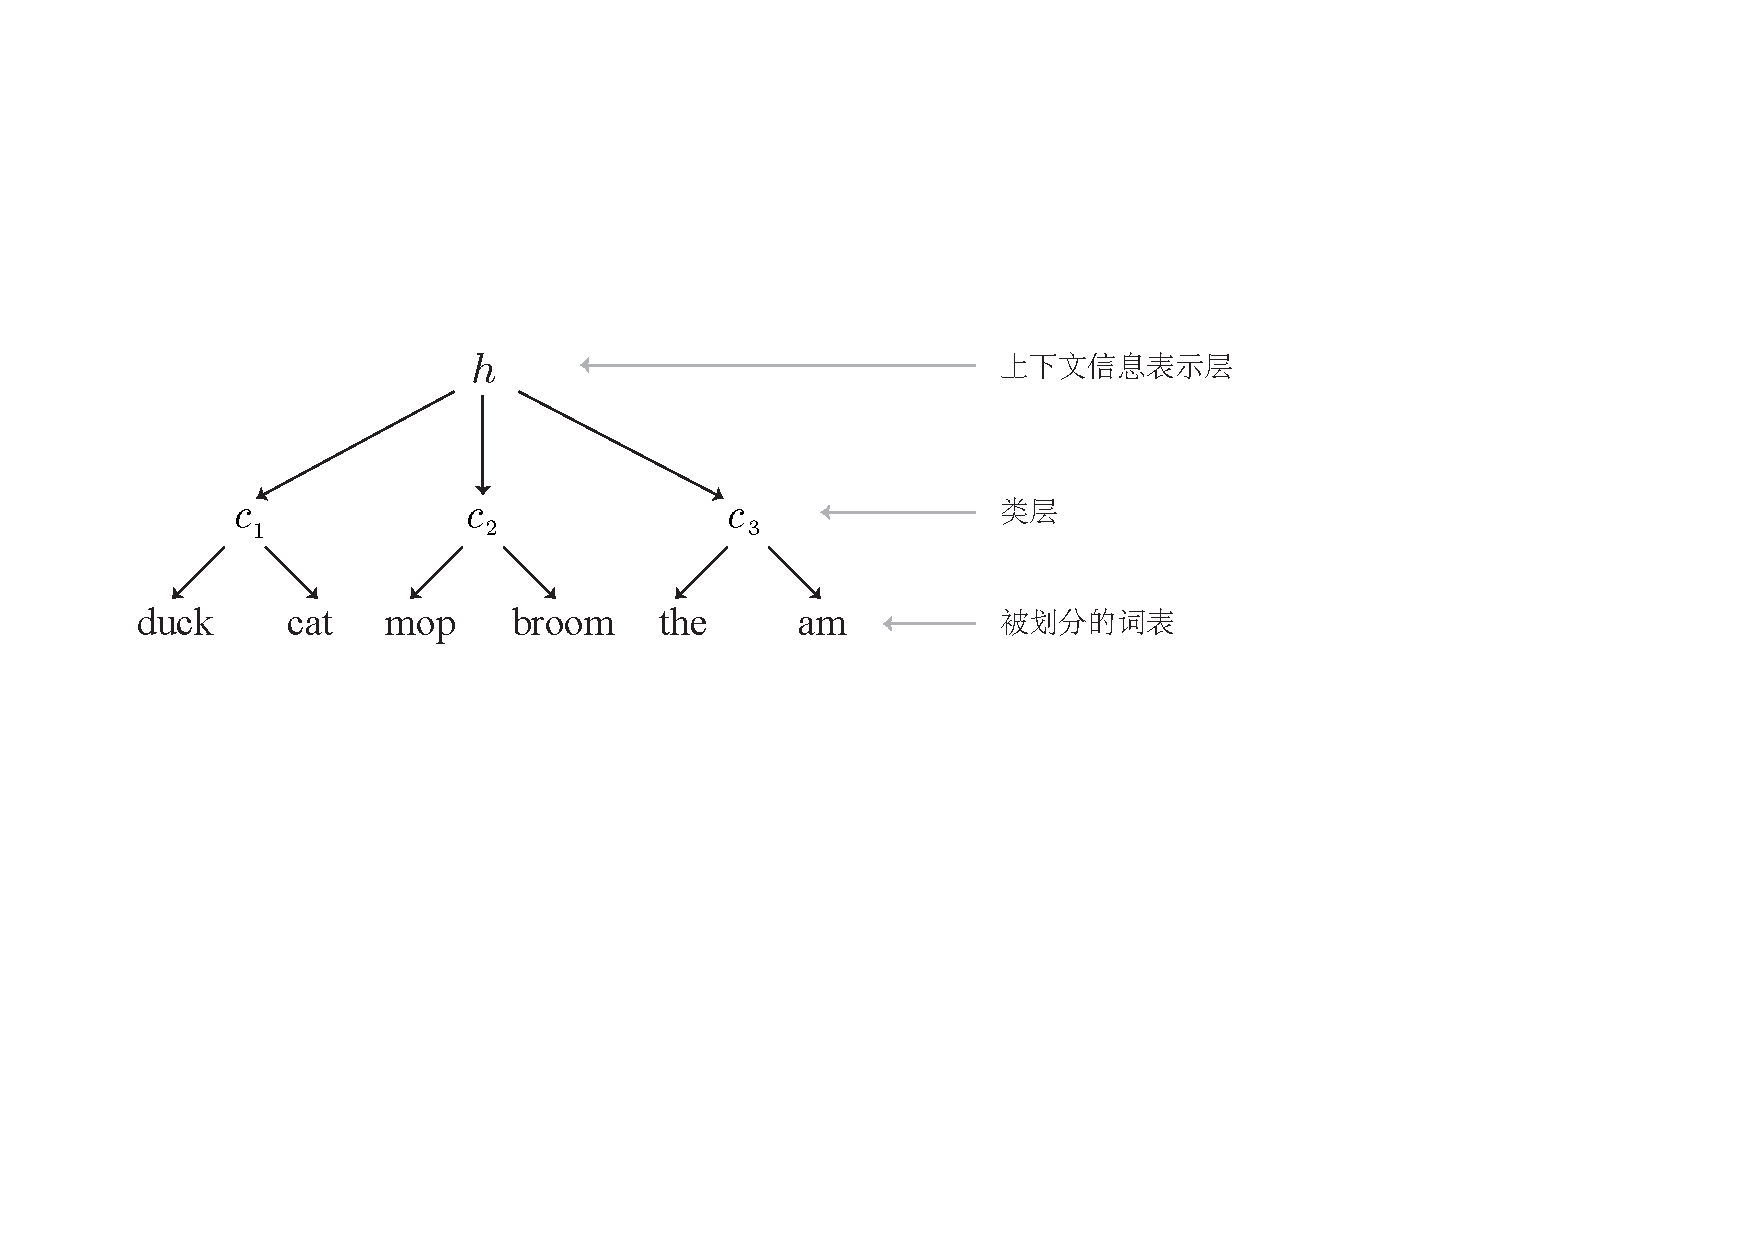
\includegraphics[width=0.7\linewidth]{./figures/case_chsm.pdf}
\caption{cHSM算法可视化模型。其中词表 \{duck,cat,mop,broom\} 被划分成:\{duck,cat\},\{mop,broom\}.}\label{fig:case_hsm}
\end{figure}



\begin{figure}
  \centering
    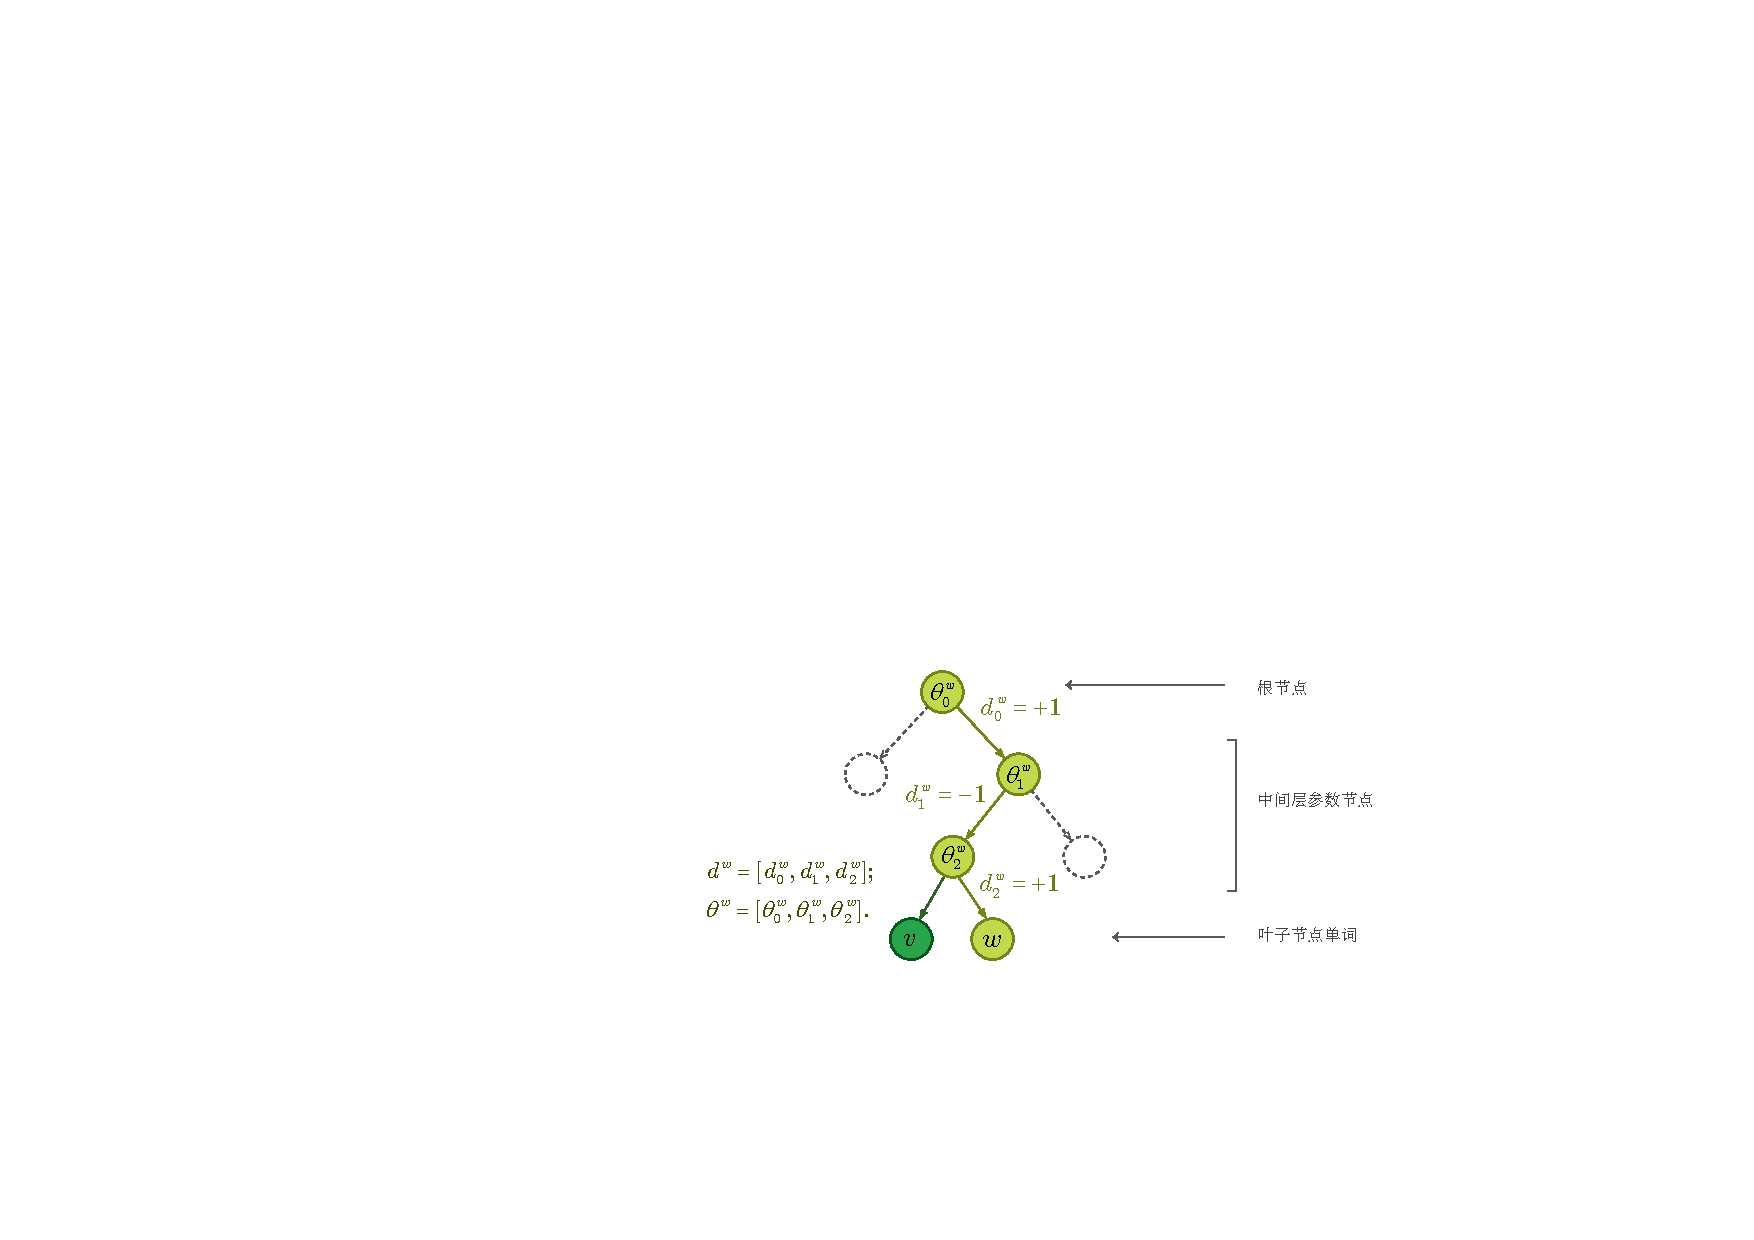
\includegraphics[width=0.75\linewidth]{./figures/thsm.pdf}
\caption{树状层次概率模型. 内部参数 $\theta_i^w$, 边 $d_i^w$ 并且单词在树的叶子节点上. 除此之外, 加粗的那条路径从根节点到叶子节点 $w$ 被定义为参数对 $(d^w,\theta^w)$。其中 $d^w$ 是一个向量, $\theta^w$ 是一个参数矩阵. 例如, $d^w=[-1,+1,-1]$ , $d^{v}=[-1,+1,+1]$.}\label{fig:tree_hsm} %
\end{figure}

 \begin{equation}
p(d^w_i|\theta_{i}^w,h) =\sigma(\theta_{i}^w h)^{d_i^w}\times[1-\sigma(\theta_{i}^w h)]^{1-{d_i^w}},d_i^w \in [0,1]
\end{equation}
 \begin{equation}
p(d^w_i|\theta_{i}^w,h) =\sigma(\theta_{i}^w h)^{d_i^w}, d_i^w \in [-1,1]
\end{equation}
\begin{equation}
p(d^w_i=\pm 1|\theta_{i}^w,h) = \sigma({d_i^w}\theta_{i}^w h)
\end{equation}

一个单词的概率 $w$:
\begin{equation}\label{equ:pw}
\begin{split}
 \log p(w|h)=&\log\prod_{i=0}^{l^w-1} p(d^w_i|\theta_{i}^w,h) = \sum_{i=0}^{l^w -1} \log\sigma(d_i^w \theta_{i}^w h)\\
 =&\log\sigma({d^w}^\top \theta^w h)=\zeta(- {d^w}^\top \theta^w h )
 \end{split}
\end{equation}
$\zeta(z)$ 表示 softplus 函数: $\zeta(z)= \log (1+\exp(z))$.
树状模型的优点:
\begin{equation}
\sum_{w\in \mathcal{V}}{p(w|h)}=\sum_{w \in \mathcal{V}}\sum_{i=0}^{l^w-1}{\sigma(d_i^w\theta_{i}^w h)}=1.
\end{equation}


\begin{figure}
  \centering
\includegraphics[width=0.45\linewidth]{./figures/softplus.png}
\caption{Softplus和ReLU函数的示意图。}\label{fig:soft}
\end{figure}

\section{关键技术或难点}

\subsection{关键技术或难点:复杂上下文建模方案}
依照上章节的分析,本章节主要介绍我们实验中所要涉及的模型,主要是各种循环神经网络的变种 \upcite{DBLP:conf/icml/JozefowiczZS15}: 普通循环神经网络节点、长短记忆网络(Long shrot-term memory, LSTM)~\upcite{DBLP:journals/taslp/SundermeyerNS15} 和门限记忆节点(Gated Recurrent Unit, GRU) \upcite{DBLP:conf/nips/ChungKDGCB15}。 LSTM的计算公式定于如下 \upcite{DBLP:journals/neco/HochreiterS97}:
\begin{itemize}
\item 输入门: 控制当前输入 $x_t$ 和前一步输出 $h_{t−1}$ 进入新的 cell 的信息量:$i_t=\sigma(W^i x_t+U^i h_{t-1}+b^i)$
\item  忘记门:决定是否清楚或者保持单一部分的状态$f_t=\sigma(W^f x_t+U^f h_{t-1}+b^f)$
\item  变换输出和前一状态到最新状态$g_t=\phi(W^g x_t+U^g h_{t-1}+b^g)$
\item  输出门: 计算 cell 的输出$o_t=\sigma(W^o x_t+U^o h^{t-1}+b^o)$
\item  cell 状态更新步骤:计算下一个时间戳的状态使用经过门处理的前一状态和输入:$s_t=g_t\odot i_t+s_{t-1}\odot f_t$
\item  最终 LSTM 的输出:使用一个对当前状态的 tanh 变换进行重变换:$h_t=s_t\odot \phi(o_t)$
\end{itemize}
其中$\odot$ 代表对应元素相乘(Element-wise Matrix Multiplication), 函数 $\phi(x), \sigma(x)$ 的定义如下:
\begin{equation}\label{equ:tanh}
  \phi(x)=\frac{e^x-e^{-x}}{e^x+e^{-x}},\sigma(x)=\frac{1}{1+e^{-x}}
\end{equation}

\begin{figure}
  \centering
  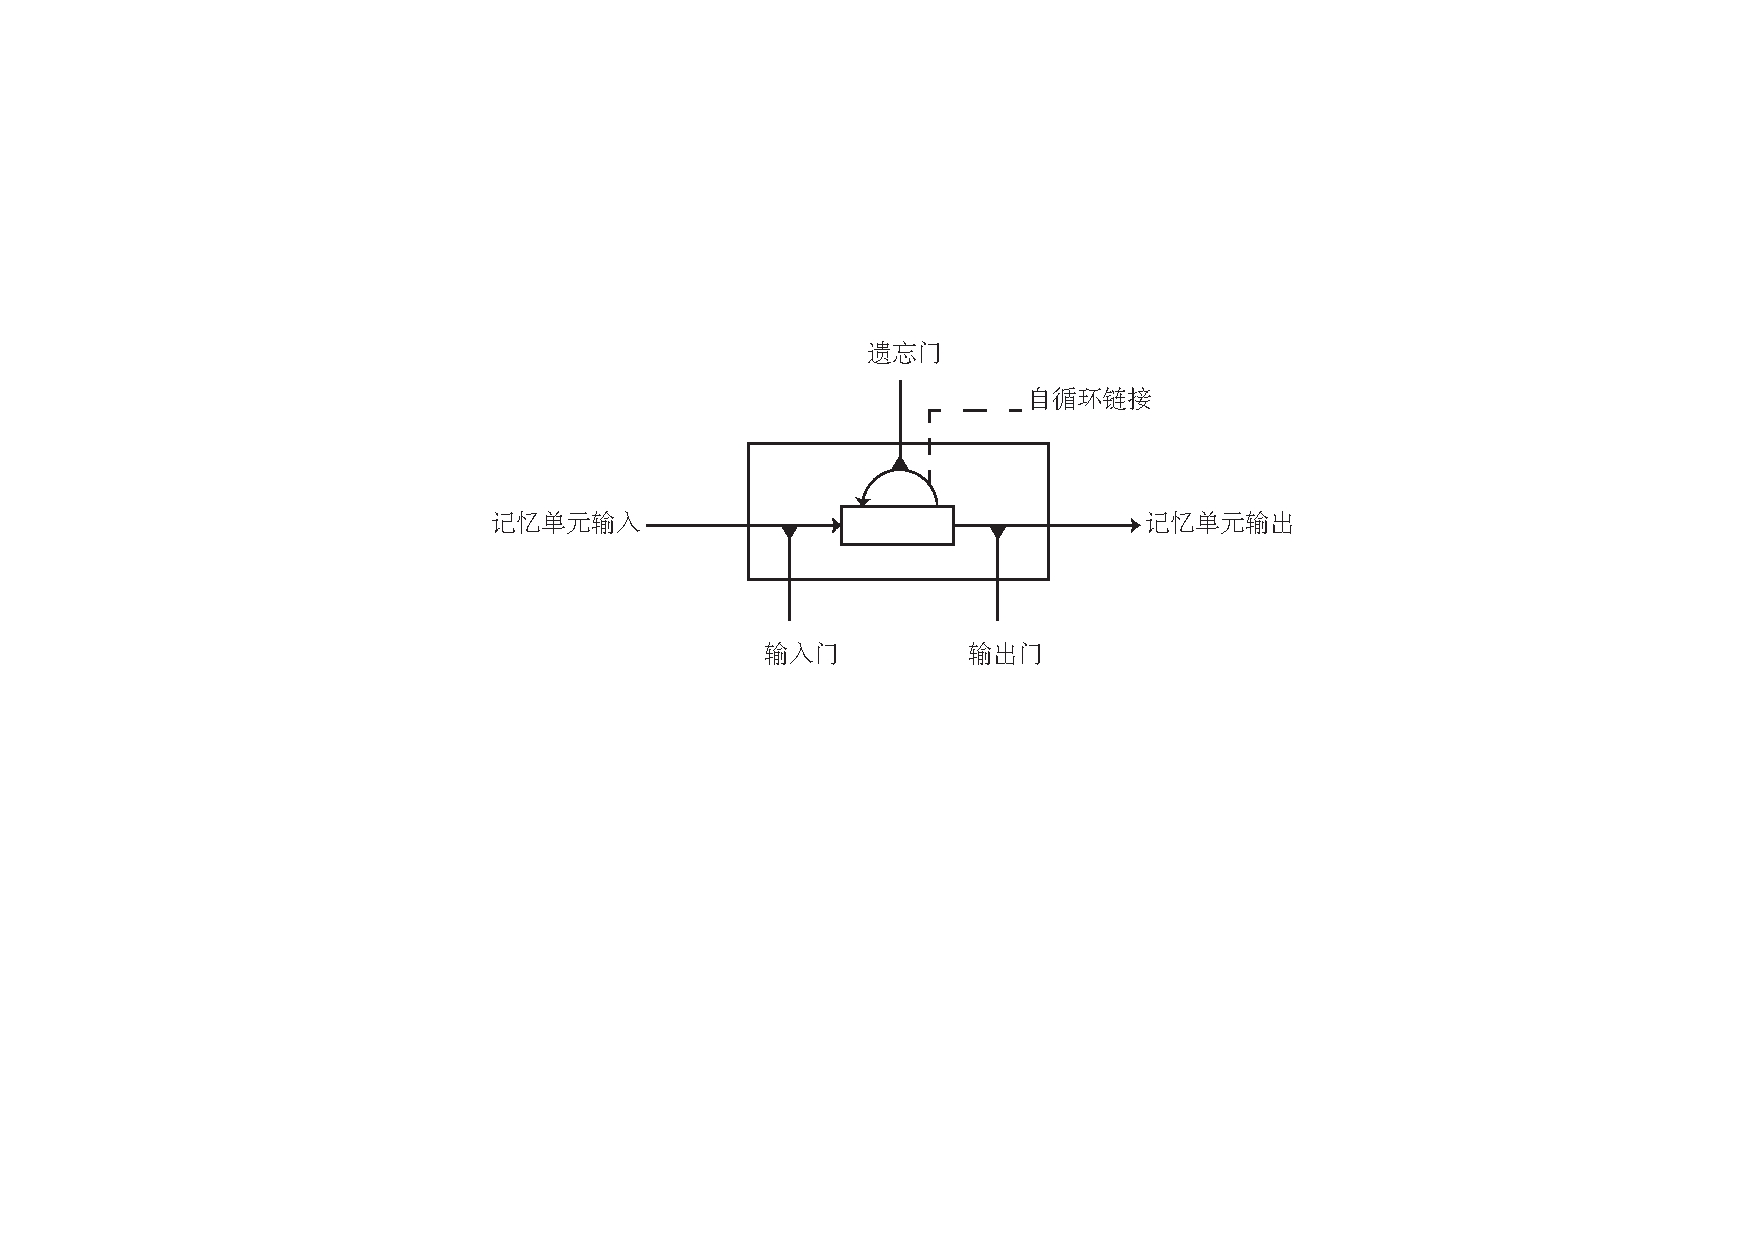
\includegraphics[width=0.7\linewidth]{./figures/lstm.pdf}
  \caption{LSTM 模型}\label{fig:lstm}
\end{figure}


GRU 可以看成是 LSTM 的变种,GRU 把 LSTM中的 遗忘门和输入门用更新门来替代。 把 cell state 和隐状态 $h_t$ 进行合并,在计算当前时刻新信息的方法和 LSTM 有所不同。 下图是GRU更新 $h_t$ 的过程\upcite{DBLP:journals/corr/Pezeshki15}, 具体定义如下:
\begin{itemize}
\item 更新门 $z_t$: 定义保存多少以前的信息: $z_t = \sigma ( W^z x_t+ U^z h_{t-1}  )$

\item 重置门 $r_t$: 决定保留多少输入信息: $r_t = \sigma(W^r x_t  + U^r h_{t-1}  )$

\item 节点内部更新值$\tilde h_t $: 其次是计算候选隐藏层(candidate hidden layer) $\tilde h_t$,这个候选隐藏层 和LSTM中的$\tilde c_t$是类似,可以看成是当前时刻的新信息,其中$r_t$用来控制需要 保留多少之前的记忆,如果$r_t$为0,那么$\tilde h_t$只包含当前词的信息:$\tilde h_t  = \tanh (W^h x_t  + U^h(h_{t-1} \odot r_t) )$

\item 隐藏层输出值$h_t$: 最后$z_t$控制需要从前一时刻的隐藏层 $h_{t-1}$ 中遗忘多少信息,需要加入多少当前 时刻的隐藏层信息$\tilde h_t$,最后得到$h_t$,直接得到最后输出的隐藏层信息, 这里与LSTM的区别是GRU中没有 输出门:$h_t = (1-z_t)\odot \tilde h_t  + z_t \odot h_{t-1}$
\end{itemize}
如果重置门接近0,那么之前的隐藏层信息就会丢弃,允许模型丢弃一些和未来无关 的信息;更新门 控制当前时刻的隐藏层输出$h_t$需要保留多少之前的隐藏层信息, 若$z_t$接近1相当于我们之前把之前的隐藏层信息拷贝到当前时刻,可以学习长距离依赖。 一般来说那些具有短距离依赖的单元重置门比较活跃(如果$r_t$为1,而$z_t$为$0$ 那么相当于变成了一个标准的RNN,能处理短距离依赖),具有长距离依赖的单元更新门比较活跃。

\begin{figure}
  \centering
  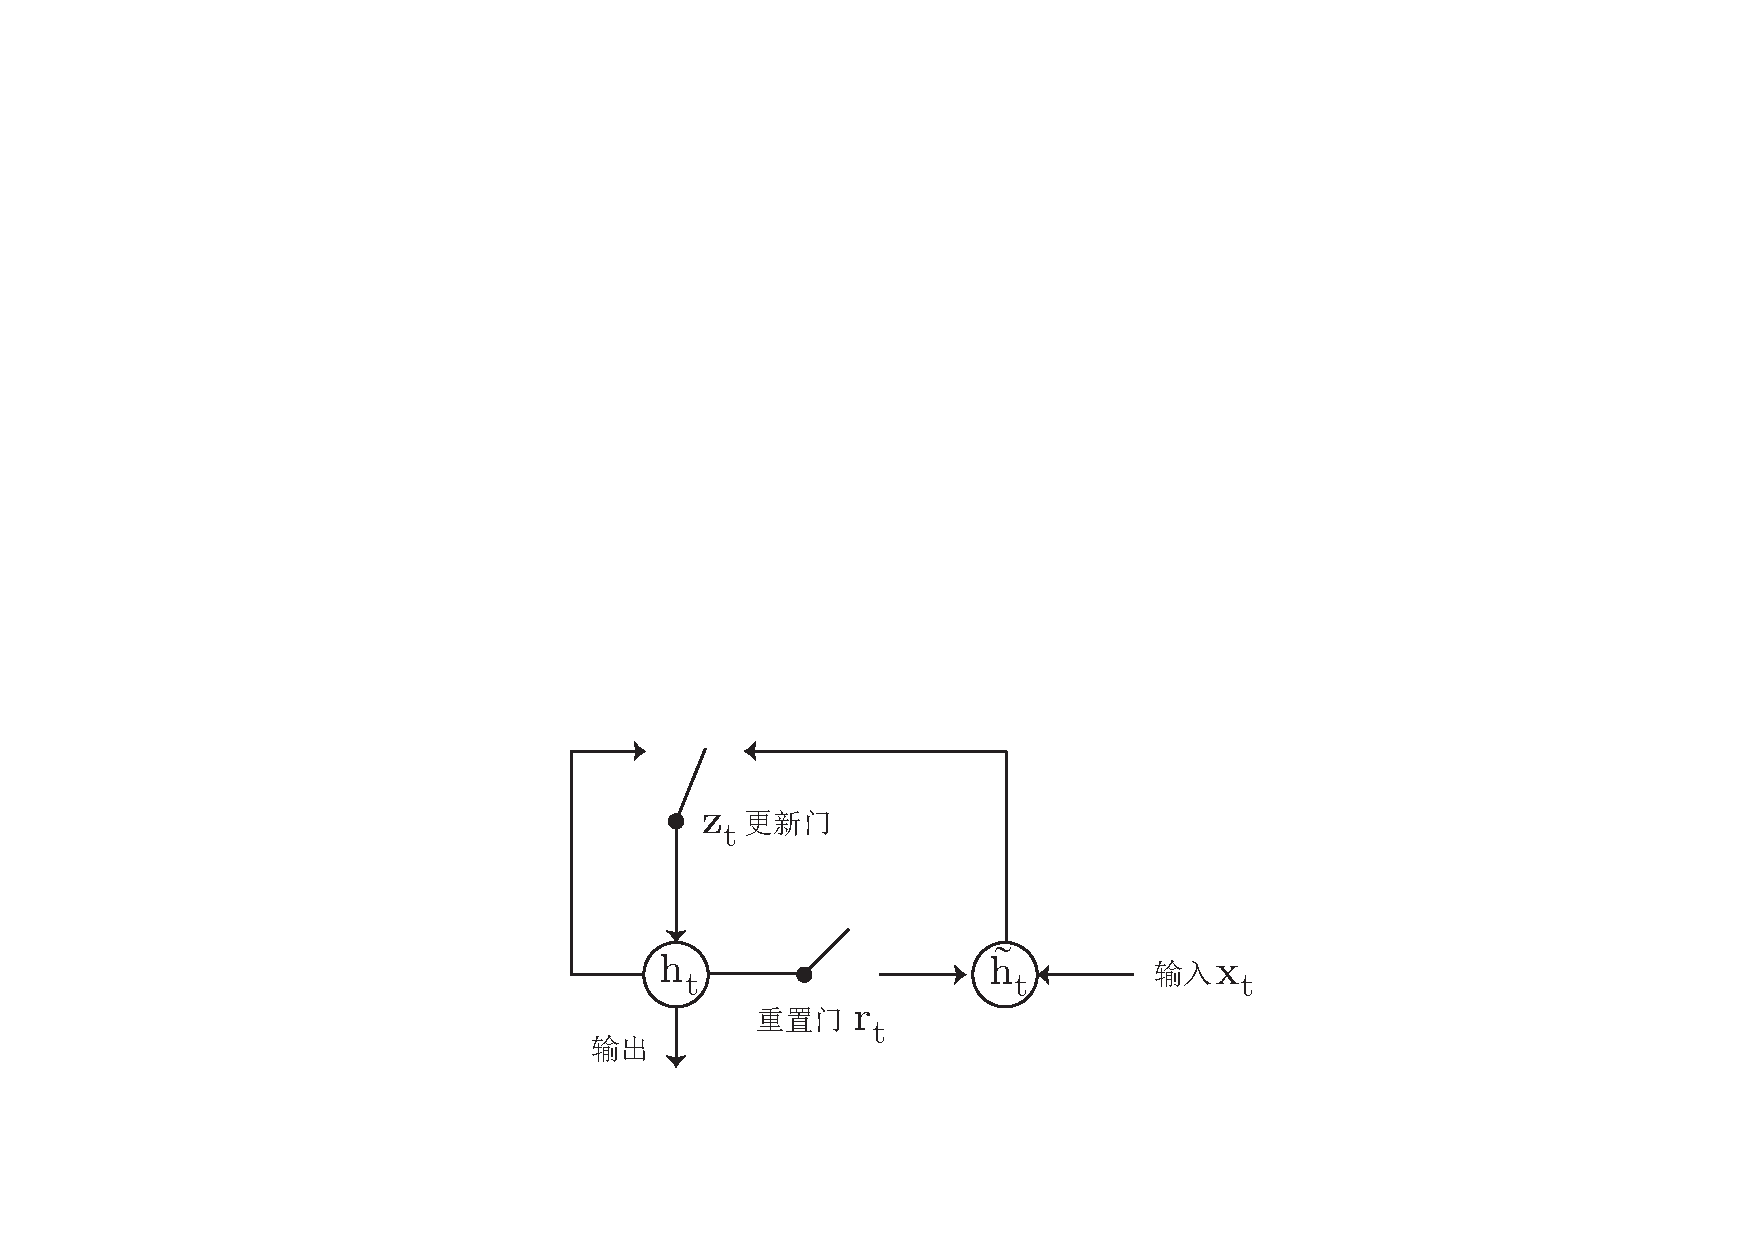
\includegraphics[width=0.45\linewidth]{./figures/gru.png}
  \caption{GRU模型示意图}\label{fig:gru}
\end{figure}


\subsection{关键技术或难点:层次概率模型}
大词表问题,主要是对softmax如何建模的问题。在本课题中,我们探讨 cHSM 和 tHSM 两种不同的方案所带来的影响和优劣。

假设语料中的每一个词样本属于且只属于一个类,在此基础上计算词样本在语料中的分布时,可以先计算类的概率分布,然后在所属类上计算当前词的概率分布,于是可将公式.~\ref{eq:softmax} 转化为:
  \begin{equation}
  \begin{split}
p(w|h)=&p^c(\mathcal{C}(w)|h)\cdot p^w(w|\mathcal{C}(w),h) , w\in \mathcal{C}(w),\\
&\mathcal{V}=\bigcup _{i = 1}^\mathcal{C}{c_i},\quad  c_i \bigcap c_j=\phi, \text{若}\quad i\ne j, \\
\end{split}
\end{equation}
此时,训练一个词样本的计算复杂度正比于: $O =HC$。 式中,$C$ 为语料中所有词的分类数,可根据语料中词的词频进行划分。 当$C$ 取$1$ 或取词典大小$V$ 时,此结构等同于标准的RNN 结构。 由于$C \ll V$,该结构训练的softmax 降低了计算复杂度。


\chapter{模型}

\begin{figure}[t]
  \centering
  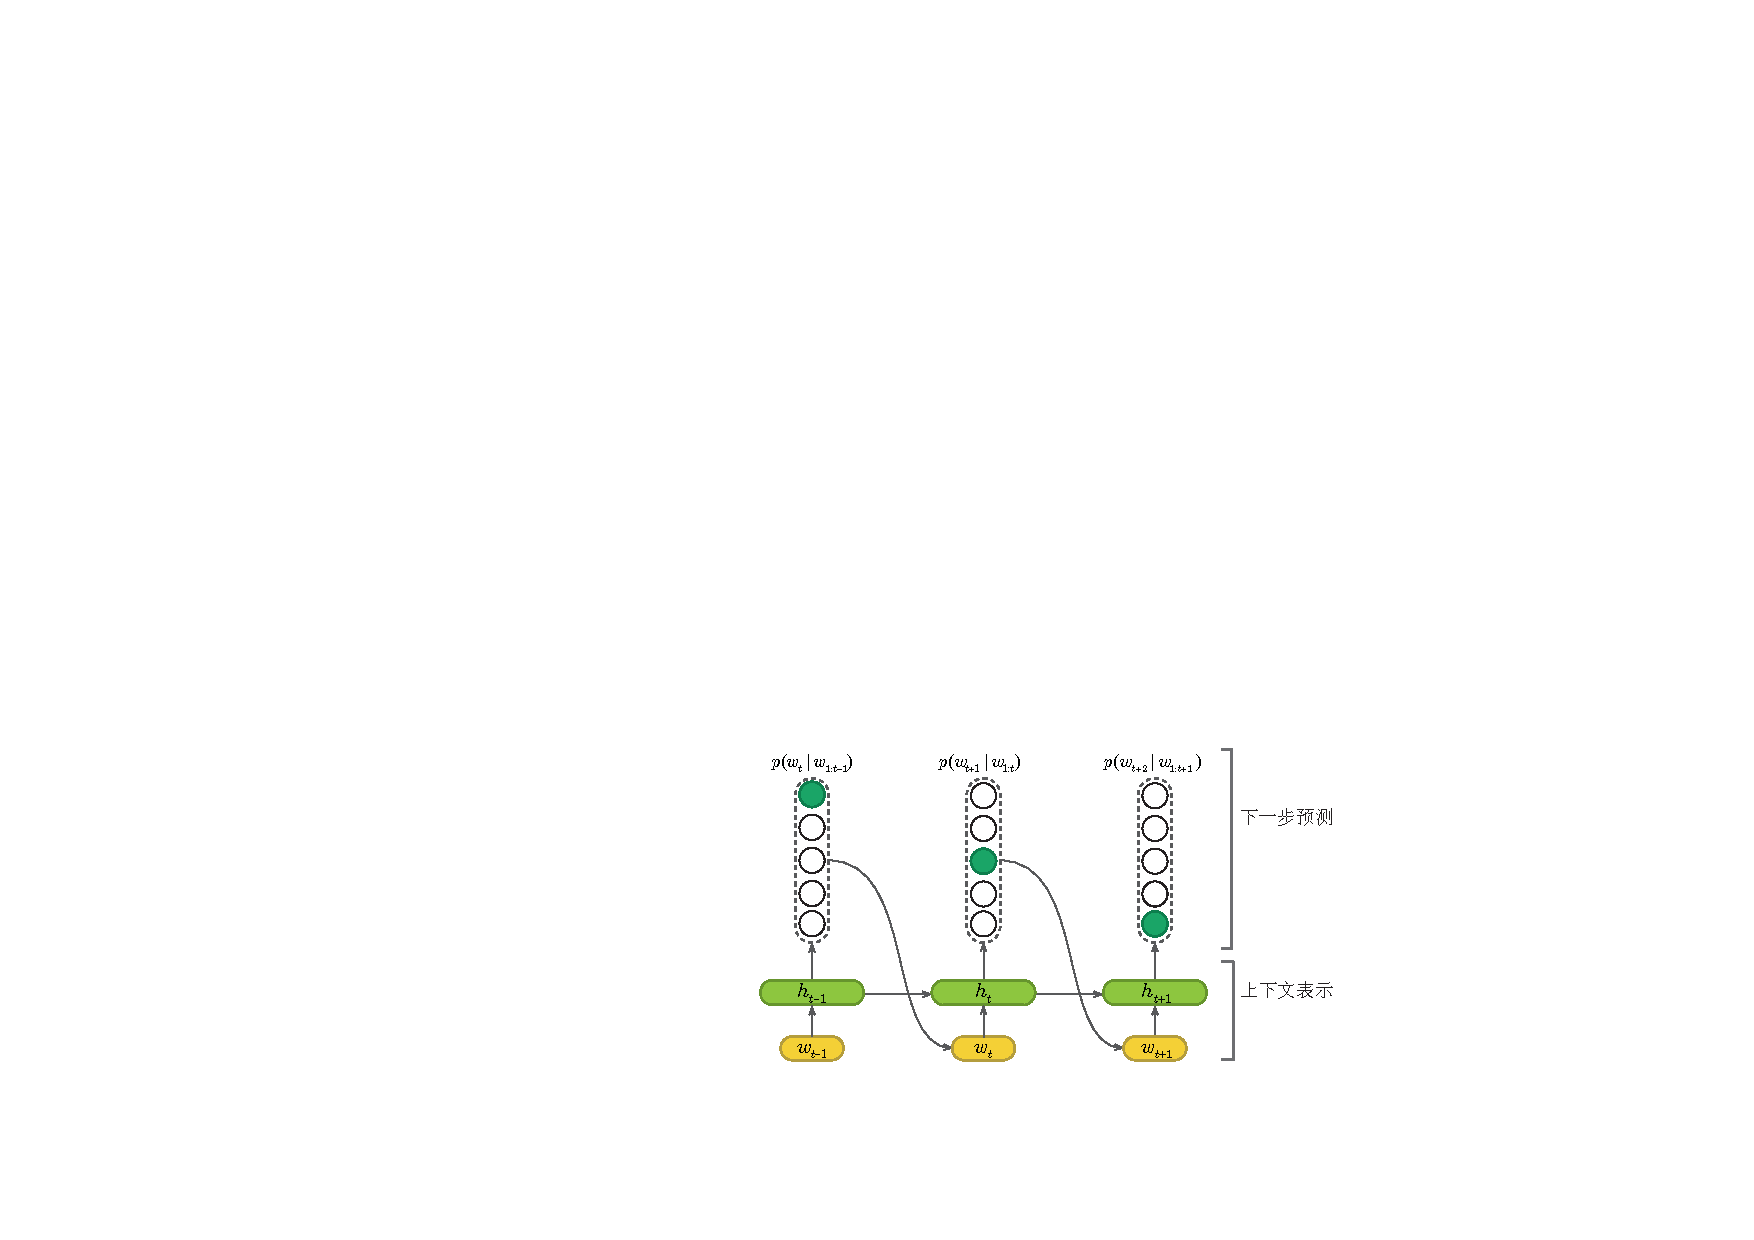
\includegraphics[width=0.7\columnwidth]{./figures/lm.pdf}
  \caption{Visualisation of Recurrent Neural Language Model. Every sentence is wrapped with start (i.e., $\langle s\rangle$) and end (i.e., $\langle /s\rangle$) tokens. Before predicting the next utterance $w_{t+1}$, the input of recurrent unit is received from the last hidden state $h_{t-1}$ and current word $w_t$.}
  \label{fig:lm}
\end{figure}

\section{模型二}
\begin{figure}[!t]
%\setlength{\abovecaptionskip}{0pt}
%\setlength{\belowcaptionskip}{0pt}
  \centering
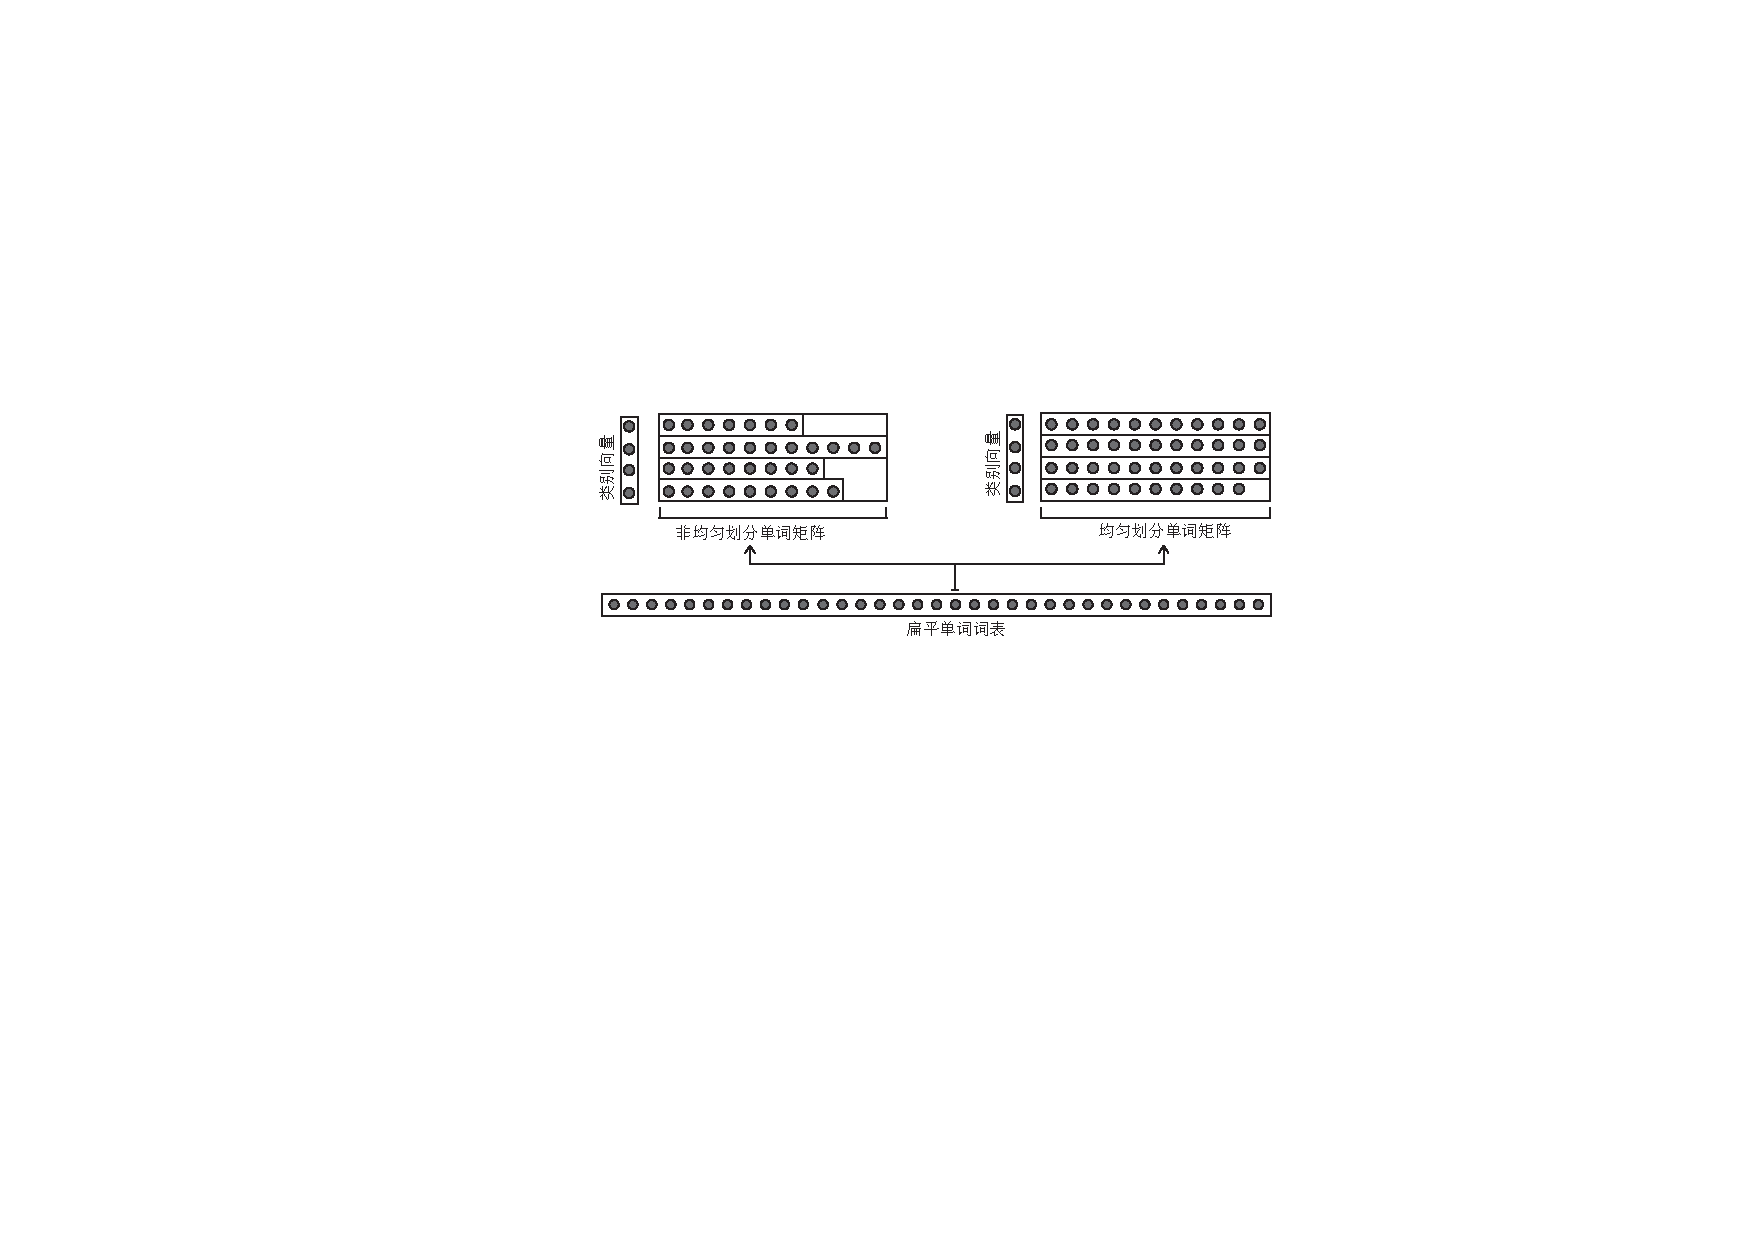
\includegraphics[width=0.85\linewidth]{./figures/chsm-simple.pdf}
\caption{Visualisation of two partition algorithms with class-based hierarchical softmax. The flatten vocabulary can be formed into upper right matrix, where the size of matrix should be greater or equal to the vocabulary and no external mask is needed.
Besides, the flatten vocabulary can be formed into upper left matrix, where external mask is needed and the composition of this matrix is depended on partition algorithms.}\label{fig:chsm}
\end{figure}
\begin{algorithm}[t]
\caption{Exact $\arg\max$ algorithm for cHSM.}\label{alog:exact}
\KwData{ Last hidden layer output $h$;}
\KwResult{ The predicted best candidate word $w$.}
 $\hat y^o=\arg\max_o{\log p^o(w| c,h)}$ \tcp*[r]{select best candidates in every group}
 $\tilde y^c=\arg\max_c{(\log p^c(y^c|h)+\log p^w(\hat y^w|\hat y^c,h))}$\tcp*[r]{calculate best candidate}
 alter $(\tilde y^c,\hat y^o[\tilde y^c])$ with word $w$ by looking-up table $\Gamma'$ \;
 \Return $w$ \;
\end{algorithm}



\begin{algorithm}[t]
\SetAlgoLined
\KwData{Hidden layer output $h$;}
\KwResult{ The predicted word $w$. }
 $\mathtt{path}$=[] \;
\While(\tcp*[h]{Search every layer}){$k \le \log \mathcal{V}$ }{
\eIf{$p(d_{k} |\theta_{k},h) \ge 0.5$ }{
 $k$= left child of node $k$ \tcp*[r]{左分支}
}{
 $k$= right child of node $k$ \tcp*[r]{右分支}
}
 $\mathtt{path}$.append($k$) \tcp*[r]{append $k$ to path list}
}
 alter $\mathtt{path}$ with word $w$ by looking-up table $\Gamma$.\;
 \Return $w$ \;
\caption{Greedy Layer-wise Argmax}\label{alog:greed_argmax}
\end{algorithm}


\chapter{语言模型实验及实验结果分析}
在前面两章中,本文按照章节分别介绍本文中使用的方法具体过程。在本章中,本文将会展示并行层次概率计算算法的实验结果,并且在第二小节中展现实验结果,以及与其他加速算法的对比。
\section{实验数据集}
\begin{table}
  \centering
  \caption{WikiText-2, WikiText-103 和 One Billion Words 数据集统计指标。 Number of tokens for train, valid and test, vocabulary size, and fraction of out-of-vocabulary (OOV) rate.\label{tab:dataset}}
\begin{tabular}{llrrrrr}
\toprule
数据集& 类型& 文章数 & 句子数量 &  单词数量 &词表大小 & OOV (\%) \\ \midrule
\multirow{3}{*}{Wikitext-2} &训练集& 600 & 36,718 & 2,088,628 & \multirow{3}{*}{33,278} & \multirow{3}{*}{2.6\%} \\
&验证集& 60 &3,760 & 217,646  & &\\
&测试集& 60 & 4,358 & 245,569 & &\\
\midrule
\multirow{3}{*}{Wikitext-103} &训练集& 28,475 &  1,801,350 &  103,227,021 & \multirow{3}{*}{267,735} & \multirow{3}{*}{0.4\%} \\
&验证集& 60 &3,760 & 217,646  & &\\
&测试集& 60 & 4,358 & 245,569 & &\\
\midrule
\multirow{3}{*}{One Billion Word} &训练集& --- &30,301,028&768,646,526&   \multirow{3}{*}{793,471} &   \multirow{3}{*}{0.28\%} \\
 &验证集& --- &  6,075 &   153,583 &&\\
 &测试集 & --- &  6,206 &   159,354 &&\\
\bottomrule
\end{tabular}
\end{table}
\section{评价指标}
\begin{equation}\label{equ:ppl}
   \mathrm{PPL}(w_1,\cdots,w_T)=\sqrt[T]{\frac{1}{\prod_{t=1}^T p(w_t|w_{1:t-1})}}
\end{equation}

\begin{equation}\label{equ:wer}
  \mathrm{WER} = \frac{\text{插入单词数 + 删除单词数 + 替换单词数}}{\text{全部单词数量}}
\end{equation}

\section{实验分析}
\begin{figure}
%\setlength{\abovecaptionskip}{0pt}
%\setlength{\belowcaptionskip}{0pt}
  \centering
  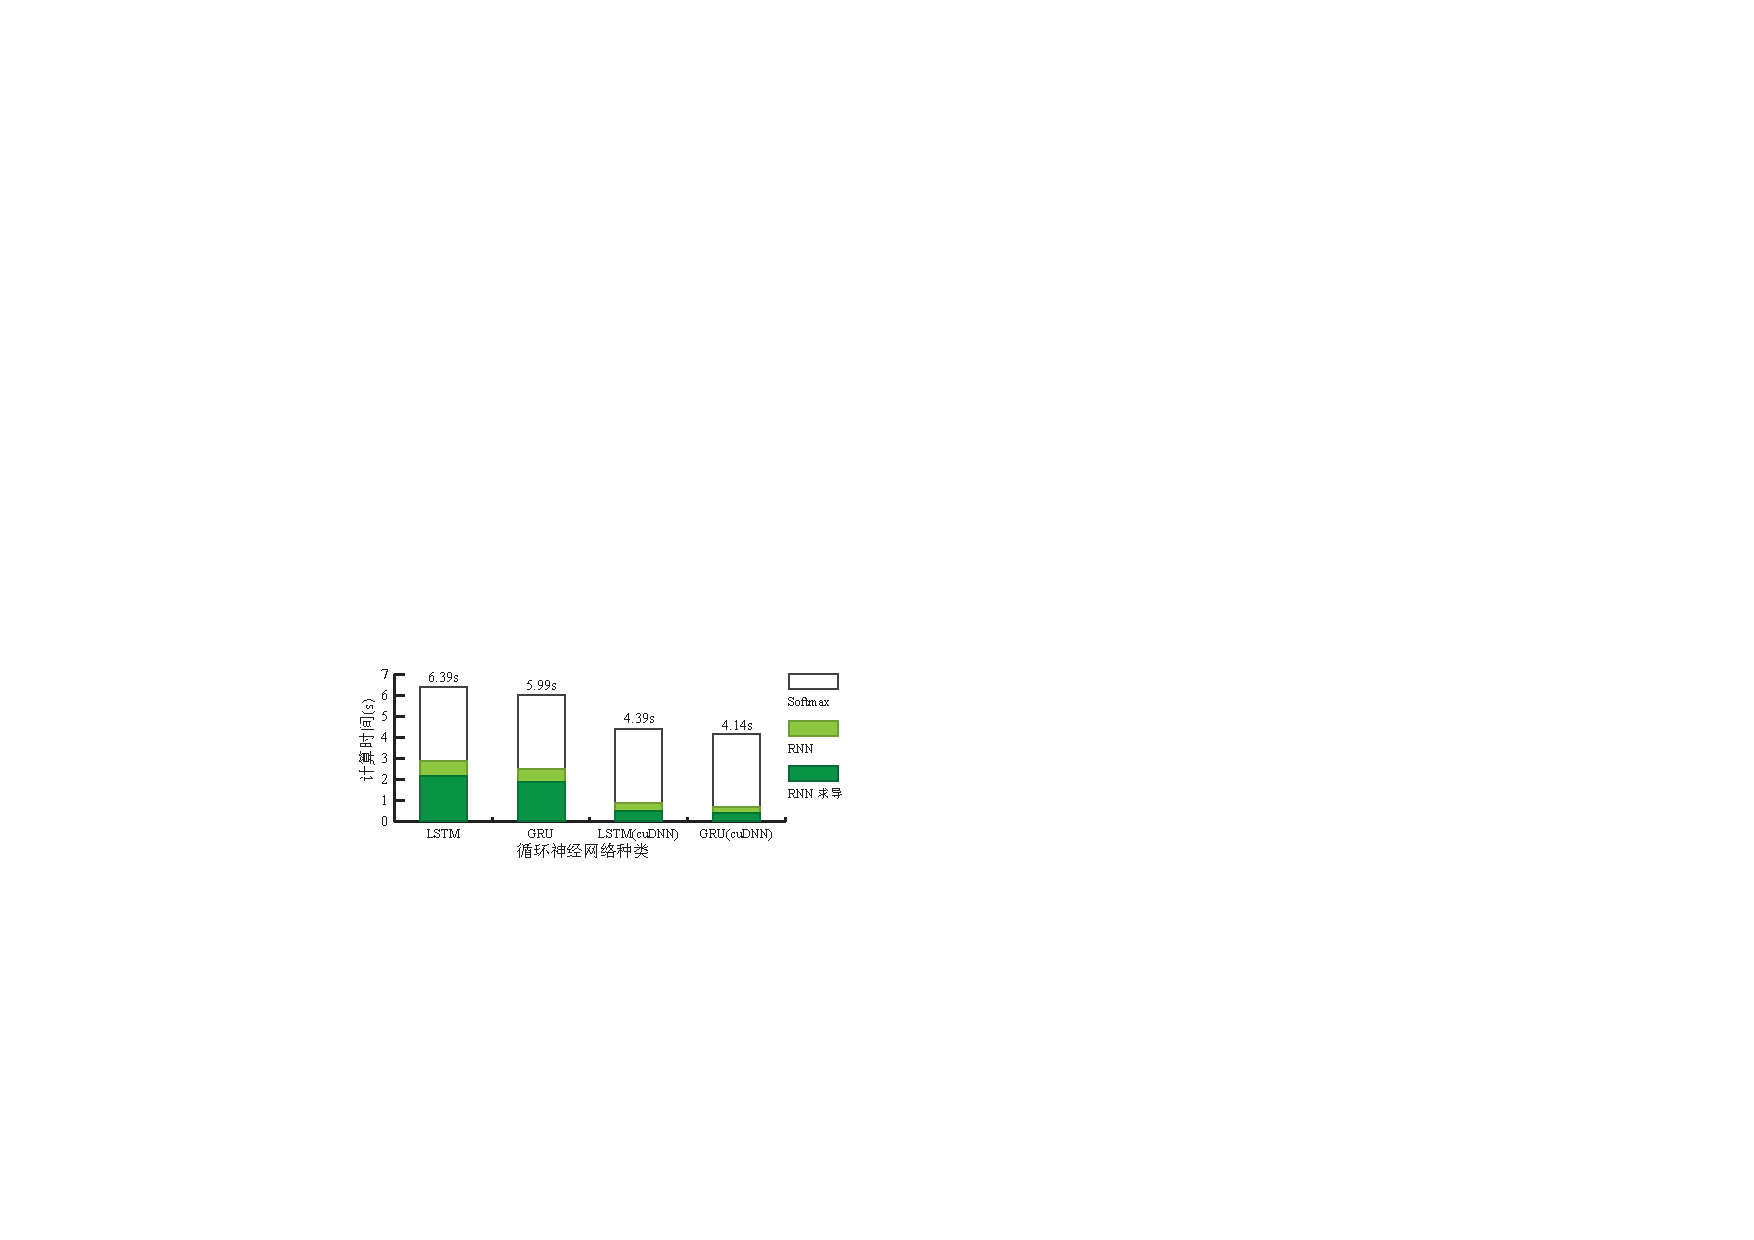
\includegraphics[width=0.6\columnwidth]{./figures/rnn_timing.pdf}
  \caption{Calculation Time of three modules with different recurrent cells on the Wikitext-103 dataset.}\label{fig:rnn_timing}
\end{figure}
\begin{figure}
%\setlength{\abovecaptionskip}{0pt}
%\setlength{\belowcaptionskip}{0pt}
  \centering
  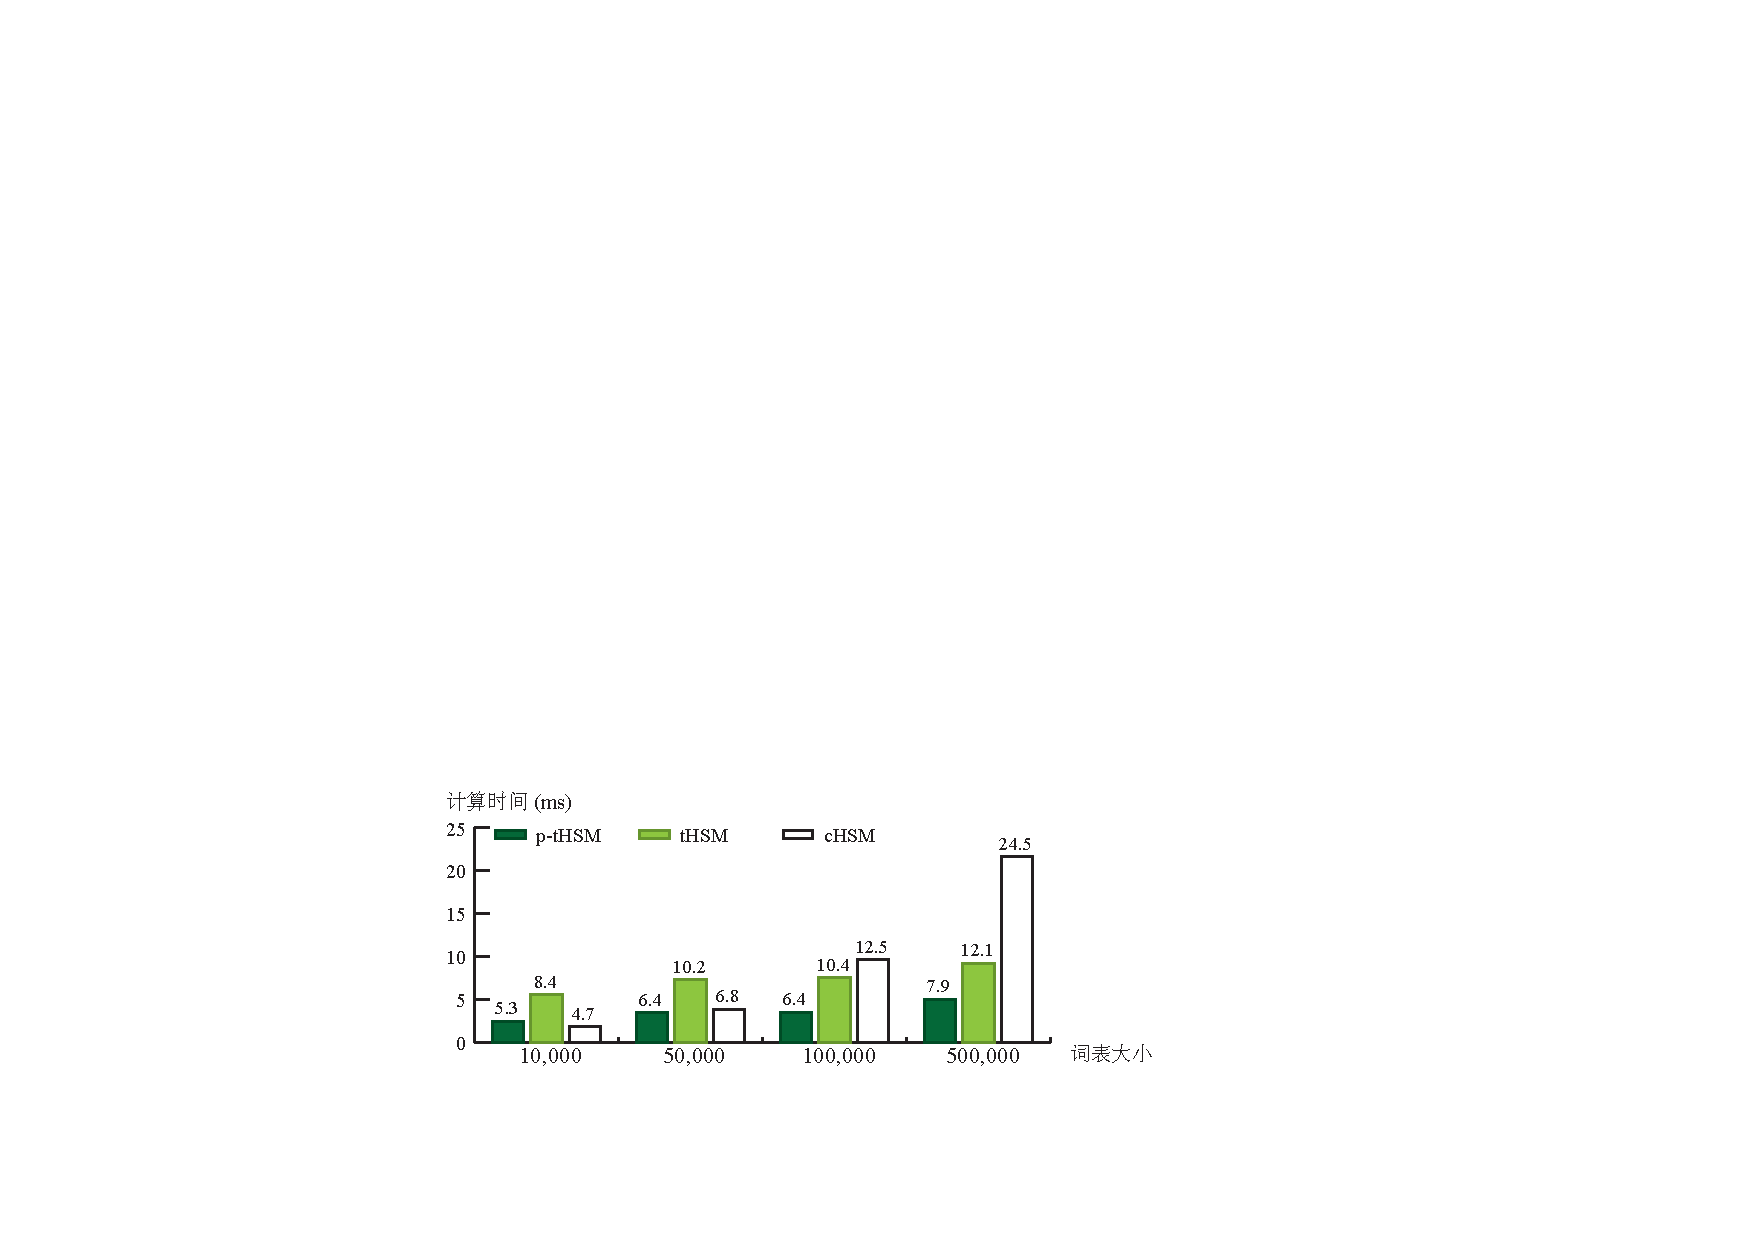
\includegraphics[width=0.6\columnwidth]{./figures/all_time.pdf}
  \caption{Scalability of cHSM, tHSM and p-tHSM algorithms with relevance to the vocabulary size.}\label{fig:hsm_benchmark}
\end{figure}
\begin{table}[!t]
%\setlength{\abovecaptionskip}{0pt}
%\setlength{\abovedisplayskip}{0pt}
  \centering
  \caption{Runtime time and memory comparison on GPUs and CPUs with WikiText-103 Dataset.\label{tab:time}}
\begin{tabular}{lccccc}
  \toprule
 \multirow{2}{*}{Methods}  &\multirow{2}{*}{Runtime Memory} &\multicolumn{2}{c}{Total Time (ms)} & \multicolumn{2}{c}{Forward Time (ms)}   \\
   \cmidrule(lr){3-4}  \cmidrule(lr){5-6}
	& & CPU&GPU & CPU& GPU \\ \midrule
Softmax & $\mathcal{|HV|}$ &510.4  &262.1&352.2& 62.9 \\
cHSM    & $2\mathcal{|H|\sqrt{|V|}}$&506.5  &\textbf{40.6}&28.7&14.6 \\
tHSM    &$\mathcal{|H|}$&1,004.0 &444.4 & 8.1&  5.6   \\
p-tHSM  &$\mathcal{|H|\log{|V|}}$ &\textbf{383.5}&	86.4 &\textbf{7.0}&	\textbf{1.4} \\
  \bottomrule
\end{tabular}
\end{table}


\begin{table}[t]
%\setlength{\abovecaptionskip}{0pt}
%\setlength{\abovedisplayskip}{0pt}
  \centering
  \caption{在Wikitext-2数据集上,cHSM 算法采用不同聚类算法的PPL 和 WER 结果 .\label{table:clustering}}
  \begin{tabular}{lclccc} \toprule
聚类算法 & 均匀划分?&分支数& 训练轮数& 测试集 (PPL / WER)&耗时 (ms)\\ \midrule
  \multirow{6}{*}{Random}  &\multirow{6}{*}{是}&10/3330&145&211.15 / 78.55 &791\\
    &&20/1664&123&228.72 / 78.89&565\\
    &&40/832&103&234.36 / 79.21&321\\
    &&80/417&78&243.12 / 79.64&171\\
    &&160/208 &57&253.38 / 80.08&92\\
    &&182/183&48&268.63 / 80.11&88\\
  \midrule
  \multirow{6}{*}{Alphabet}  &\multirow{6}{*}{是}&10/3330 &141&199.01 / 78.07 &773\\
    &&20/1664 &120&211.34 / 78.23&551\\
    &&40/832 &100&238.75 / 79.02&313\\
    &&80/417 &90&241.75 / 79.34&174\\
    &&160/208 &56&248.35 / 79.62&97\\
    &&182/183&45&258.57 / 80.02&87\\
  \midrule
  \multirow{6}{*}{Unigram}   &\multirow{6}{*}{是} &10/3330&134&211.51 / 77.41 &788\\
    & &20/1664&122&220.01 / 77.71&549\\
    & &40/832&113&236.56 / 77.95&302\\
    & &80/417&91& 241.12 / 78.25&170\\
    & &160/208&55&247.25 / 79.21&93\\
    & &182/183&42&253.35 / 79.92&86\\
  \midrule
  \multirow{5}{*}{Bigram}   &\multirow{5}{*}{否}&10/3672&150&208.11 / 77.32&801\\
     &&20/1923&121&217,34 / 77.64&621\\
     &&40/1123&102&228.87 / 78.14&588\\
     &&80/572&89&246.32 / 78.43&186\\
     &&160/340&76&252.33 / 79.51&97\\
  \midrule
  \multirow{5}{*}{Syntactic}  &\multirow{5}{*}{否}&10/3612 &152&214.31 / 78.11&810\\
    &&20/1972 &130&220.19 / 78.86&633\\
    &&40/996 &101&232.33 / 79.33&543\\
    &&80/545 &89&241.34 / 79.84&179\\
    &&160/235 &70&262.34 / 80.14&134\\
  \midrule
  \multirow{5}{*}{Semantic}  &\multirow{5}{*}{否} &10/3570 &133&208.77 / 77.41&819\\
    & &20/1873 &114&218.31 / 77.78&641\\
    & &40/1092 &91&225.38 / 78.35&521\\
    & &80/561 &69&238.45 / 78.91&174\\
    & &160/244 &44&256.75 / 79.41&103\\
\bottomrule
  \end{tabular}
\end{table}
\begin{table}[t]
%\setlength{\abovecaptionskip}{0pt}
%\setlength{\abovedisplayskip}{0pt}
  \centering
   \caption{Perplexity of p-HSM algorithms with various clustering methods on Wikitext-2 Dataset.\label{table:p-thsm}}
  \begin{tabular}{lcccc} \toprule
  Methods   &Build Time&Max Tree Depth &Validation Set (PPL) & Testing Set (PPL)  \\ \midrule
  Uigram  &3min&12 &218.42& 216.05     \\
  Bigram  &35h&21& 186.23& 189.58\\
  Semantic &26h &18& \textbf{163.12} & \textbf{178.78}\\
\bottomrule
  \end{tabular}
\end{table}

\begin{table}[t]
%\setlength{\abovecaptionskip}{0pt}
%\setlength{\abovedisplayskip}{0pt}
  \centering
  \caption{Word error rate with different searching rules on Wikitext-2 dataset.\label{tab:search}}
\begin{tabular}{llccc}
  \toprule
   & Type&Time (ms)&Validation set (WER)& Testing set (WER)\\ \midrule
  \multirow{3}{*}{cHSM} &global&102& 80.00\%& 80.02\%\\
        &Algorithm~\ref{alog:exact}&63& 80.00\%& 80.02\%\\
        &Algorithm~\ref{alog:argmax}&\textbf{44}&\textbf{ 77.09\%}&\textbf{ 77.07\%}\\\midrule \midrule
        & Type&Time (ms)&Validation set (WER)& Testing set (WER)\\ \midrule
  \multirow{2}{*}{p-tHSM}  &global&161& \textbf{76.67\%}&\textbf{75.35\%}\\
        &Algorithm~\ref{alog:greed_argmax}&\textbf{30} & 79.61\%&79.32\%\\
  \bottomrule
\end{tabular}
\end{table}

\subsection{Impact of Recurrent Cells}
\begin{table}[!t]
%\setlength{\abovecaptionskip}{0pt}
%\setlength{\abovedisplayskip}{0pt}
  \centering
  \caption{Results of different recurrent cells on Wikitext-2 dataset with metrics: PPL, WER and calculation time.\label{tab:rnn}}
\begin{tabular}{lccc}
  \toprule
  \multirow{2}{*}{Recurrent Cells} & \multirow{2}{*}{Time (ms)}&Validation Set & Testing Set\\
  && PPL / WER & PPL / WER\\ \midrule
  1$\times$RNN Relu~\upcite{DBLP:journals/jmlr/GutmannH10} &176.4&260.52 / 80.00\%&238.75 / 80.02\%\\
  1$\times$RNN Tanh~\upcite{DBLP:journals/iclr/JiVSAD15}   &176.2&250.57 / 79.61\%&230.98 / 79.32\%\\
  1$\times$LSTM~\upcite{7508408}                  &\textbf{189.5}&180.98 / 77.16\%&165.60 / 76.67\%\\
  1$\times$GRU~\upcite{DBLP:journals/corr/ChungGCB14}      &191.3&\textbf{179.59 / 77.09\%}&\textbf{165.32 / 77.07\%}\\ \midrule
  2$\times$RNN Relu~\upcite{DBLP:journals/jmlr/GutmannH10} &266.3&190.52 / 73.01\%&198.75 / 73.02\%\\
  2$\times$RNN Tanh~\upcite{DBLP:journals/iclr/JiVSAD15}   &266.3&189.57 / 72.62\%&260.98 / 72.32\%\\
  2$\times$LSTM~\upcite{7508408}                  &\textbf{279.4}&164.98 / 71.17\%&165.60 / 71.67\%\\
  2$\times$GRU~\upcite{DBLP:journals/corr/ChungGCB14}      &281.2&\textbf{158.59 / 70.08\%}&\textbf{155.32 / 70.07\%}\\
  \bottomrule
\end{tabular}
\end{table}

\begin{figure}[t]
%\setlength{\abovecaptionskip}{0pt}
%\setlength{\belowcaptionskip}{0pt}
  \centering
  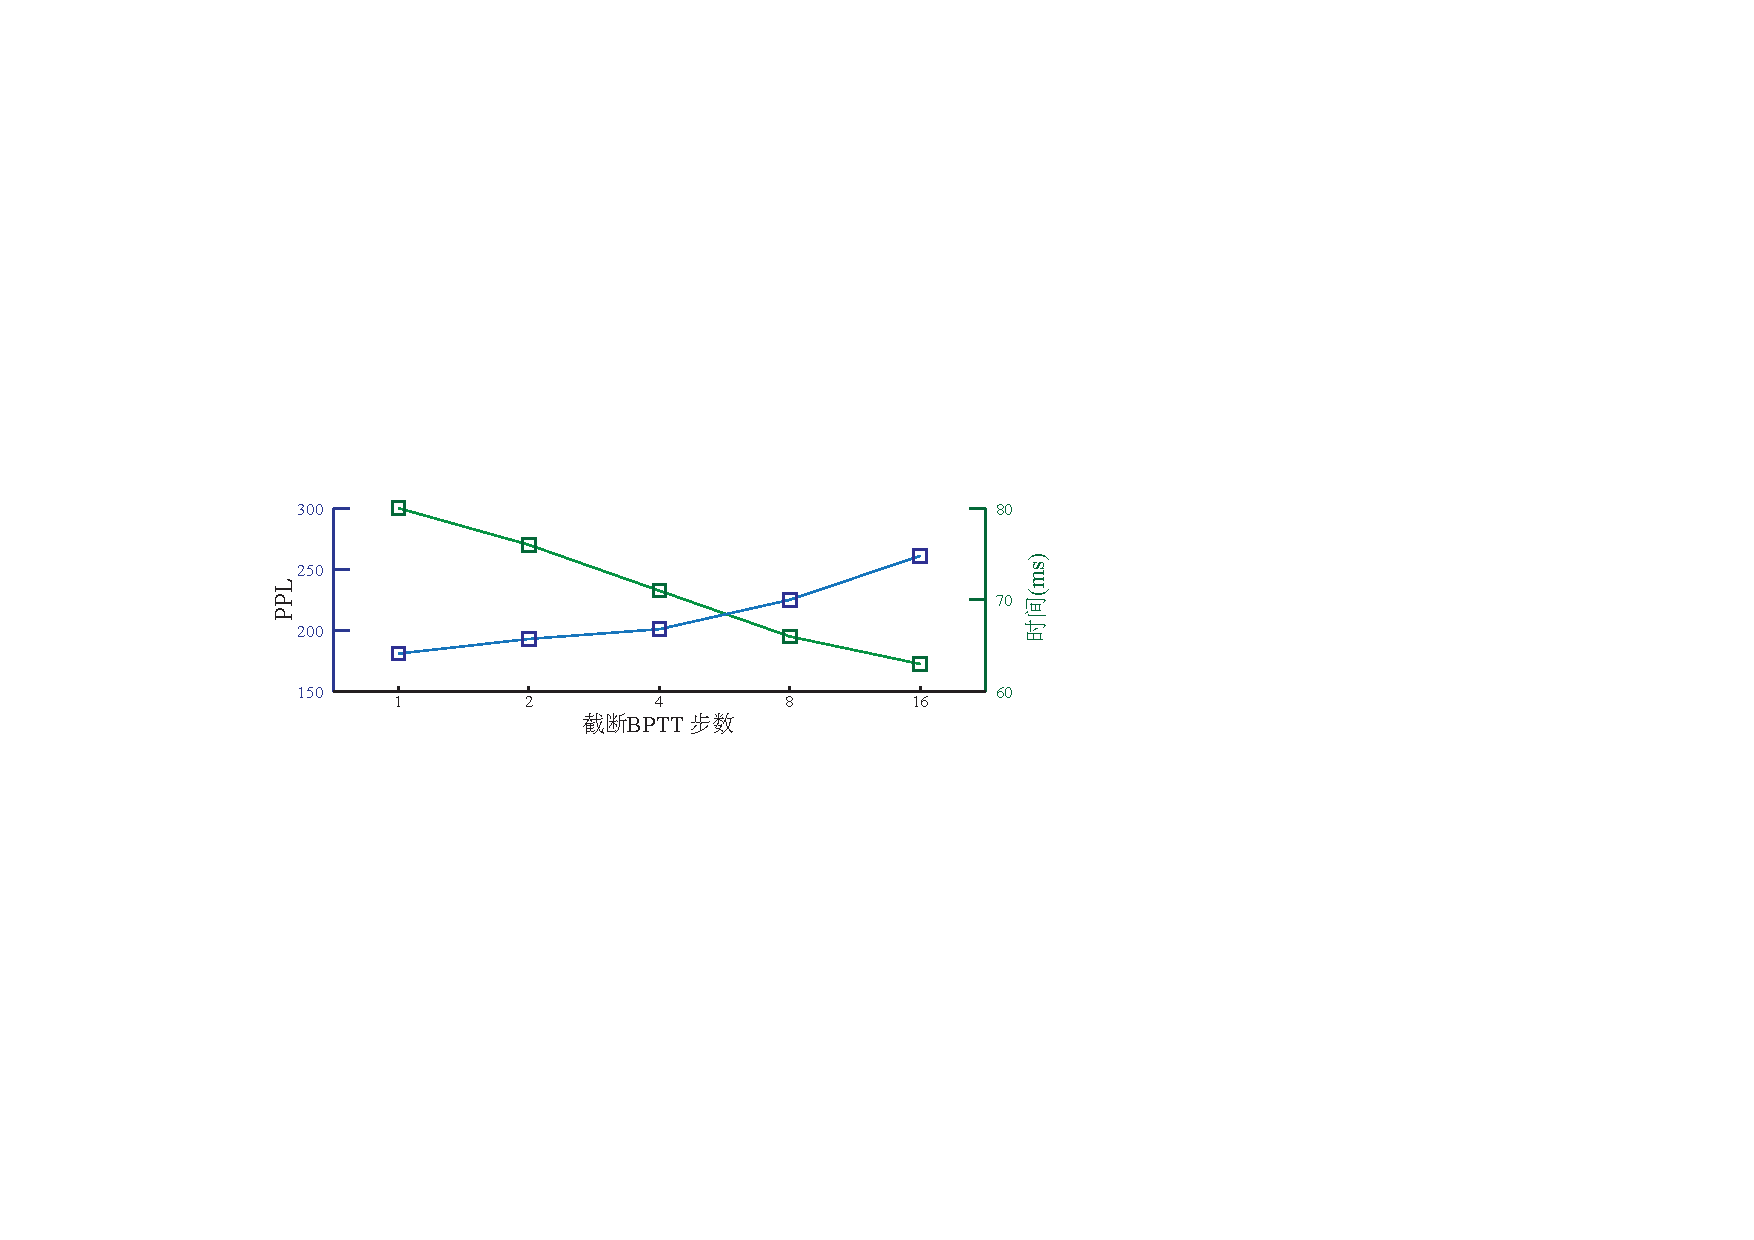
\includegraphics[width=0.65\columnwidth]{./figures/tbptt.pdf}
  \caption{Perplexity comparison of different Truncated BPTT Steps with the NCE and Blackout methods on Wikitext-2 dataset.}\label{fig:tbptt}
\end{figure}


\subsection{All Experiments Benchmark}

\begin{table}[t]
%\setlength{\abovecaptionskip}{0pt}
%\setlength{\abovedisplayskip}{0pt}
  \centering
  \caption{Perplexity and Word Error Rate on Wikitext-2,  WikiText-103 and One Billion Word Datasets.\label{tab:summary_ppl}}
\begin{tabular}{llcc}
  \toprule
数据集& 算法& 验证集(PPL/ WER) & 测试集(PPL/WER) \\ \midrule
 \multirow{2}{*}{WikiText-2}&GRU + Softmax&172.64 / 77.49\%&162.09 / 77.07\% \\
  &GRU + NCE~\upcite{DBLP:journals/jmlr/GutmannH10}&217.84 / 78.26\%&199.54 / 78.02\%\\
  &GRU + Blackout~\upcite{DBLP:journals/iclr/JiVSAD15}&221.15 / 77.72\%&199.56 / 77.50\% \\
  &GRU + cHSM + unigram~\upcite{DBLP:conf/acl/ChenGA16}&253.18 / 78.25\%&236.61 / 78.02\%\\
  &GRU + p-tHSM + unigram~\upcite{DBLP:conf/nips/MikolovSCCD13}&218.42 / 78.15\%&216.05 / 78.15\%\\
  &GRU + p-tHSM + bigram~\upcite{DBLP:journals/coling/BrownPdLM92}&186.23 / 78.15\%&189.58 / 78.15\%\\\midrule
   \multirow{2}{*}{WikiText-103} &GRU + Softmax&130.38 / 72.15\%&136.83 / 72.37\%\\
 &GRU + NCE~\upcite{DBLP:journals/jmlr/GutmannH10}&164.78 / 73.22\%&165.01 / 73.34\%\\
  &GRU + Blackout~\upcite{DBLP:journals/iclr/JiVSAD15}&163.99 / 73.18\%&162.76 / 74.22\%\\
  &GRU + cHSM + unigram~\upcite{DBLP:conf/acl/ChenGA16}&171.81 / 73.42\%&166.74 / 73.18\%\\
  &GRU + p-tHSM + unigram~\upcite{DBLP:conf/nips/MikolovSCCD13}&165.70 / 73.53\%&166.11 / 72.44\%\\
  &GRU + p-tHSM + bigram~\upcite{DBLP:journals/coling/BrownPdLM92}&164.15 / 78.15\%&163.55 / 77.85\%\\\midrule
  \multirow{2}{*}{One Billion Word} &GRU + Softmax&330.38 / 88.15\%&330.83 / 88.37\%\\
 & GRU + NCE~\upcite{DBLP:journals/jmlr/GutmannH10}&272.07 / 84.83\%&276.11 / 84.34\%\\
  &GRU + Blackout~\upcite{DBLP:journals/iclr/JiVSAD15}&268.67 / 84.23\%&266.11 / 84.18\%\\
 & GRU + cHSM + unigram~\upcite{DBLP:conf/acl/ChenGA16}&225.36 / 80.32\%&224.11 / 79.42\%\\
 & GRU + p-tHSM + unigram~\upcite{DBLP:conf/nips/MikolovSCCD13}&231.44 / 87.53\%&236.11 / 82.53\%\\
  &GRU + p-tHSM + bigram~\upcite{DBLP:journals/coling/BrownPdLM92}& 221.55 / 81.15\%&218.70 / 83.15\%\\
  \bottomrule
\end{tabular}
\end{table}


\section{总结和展望}
Mikolov曾提出使用基于二叉树的层级softmax模型来加速的训练方案,加速比能达到理论的最大速度,但是当时提出的背景是基于CPU构建的,如今越来越多的算法随着应用领域的推广,需要在并行度更高的GPU上进行计算,因此基于GPU进行建模的tHSM尚未被研究提及,需要在本文中研讨。
\section{下一阶段工作计划}
当我们使用多层分类模型的时候,我们就需要将单词按照模型的架构进行划分。其中对于cHSM模型,我们有以下策略可以使用:1) 基于词频划分类别; 2) 基于Bigram 的布朗聚类(Brown clustering) 进行划分;3)按照word-embedding 的词向量信息进行聚类。另外,我们还需要注意的是,各个类别可以包含不同的数量的单词,也可以包含数量相同的单词。对于后者,我们考虑的划分模型就是基于交换算法(Exchange Algorithm), 以此来保证获得近似的最优解。

\subsection{存在的问题}
目前存在的问题主要是两点:模型仍然计算很复杂需要使用更底层语言来加速计算,和目前采用的聚类算法比较费时间。

由于我们选择的建模平台是python平台,好处是可以使用许多现成的已有的框架。并且python语法简单,矩阵计算库numpy和scipy更成熟,便于调试。另一方面,我们采用的建模语言是theano框架,它的底层计算都是调用BLAS计算库,或者直接调用基于GPU的CUDA的CuBLAS计算库。虽然这样做便于在前期模型建立阶段能方便尝试各种设计方案,但是他的计算瓶颈在python解释器对代码的缓慢执行,所以如果能将部分模型组件使用CUDA语言重写。那样的话,我们的模型能接受一定的组合排列的可能性,同时计算速度能得到极大提升。这也是许多目前流行框架发展的方向,有些框架更超前。例如MXNET直接使用C++语言建立深度模型,他的计算效率也是目前已知的框架中最快的。因此,考虑到目前的thenao计算瓶颈,我们想将RNN的框架使用CUDA语言重构,基于CuDNN库开发的样板,帮助我们在他基础上改进。

另一方面,目前采用的聚类算法计算非常费时,尤其是当我们希望进行多层次聚类的时候,我们需要花费数周时间来获得结果。这样的缓慢的计算效果是无法接受的,经过针对代码的调试,我们发现计算瓶颈在算法初始化的时候,计算两两单词之间的距离,它花费了90\%的计算时间。如果能存在有效的初始化算法,而不是挑选尽可能高精度的聚类模型,那么实验进度和试验结果就可以针对多组参数调试。
\subsection{尚未完成的工作}
\begin{enumerate}
\item 大规模实验数据分析验证算法;
\item 优化模型速度,用底层语言封装模型,以达到最好的效果;
\item 实验和评价不同聚类算法的效果;
\item 讨论和研究不同语言模型优化方案的优缺点,以及使用场景。
\end{enumerate}
\subsection{解决问题的技术思路或措施}
\begin{enumerate}
\item 大规模实验数据分析验证算法:目前已经找到三个标准文本数据集,需要重写数据处理算法,这样保证模型能正常运算和收敛;
\item 优化模型速度,用底层语言封装模型,以达到最好的效果:学习CUDA语言,并着手构建基于深度学习的模型框架;
\item 实验和评价不同聚类算法的效果:调研可用的层次聚类算法并进行测试和实验检验;
\item 讨论和研究不同语言模型优化方案的优缺点,以及使用场景:提出不同的实验评价指标,观察不同模型的结果,并分析其背后的原因。
\end{enumerate}
% 参考文献
\cleardoublepage
\phantomsection
\addcontentsline{toc}{chapter}{参考文献}
\nocite{*}
\bibliography{thesis_reference}
\cleardoublepage

% 附录
%\appendix

% 附页标题样式
\backmatter

% 附页
% !Mode:: "TeX:UTF-8"
\chapter{攻读硕士学位期间取得的学术成果}
% 此处标题及内容请自行更改
\noindent 发表论文:

\noindent 1. \textbf{Nan Jiang}, Wenge Rong, Min Gao, Yikang Shen and Zhang Xiong. Exploration of Tree-based Hierarchical Softmax for Recurrent Language Models[C]. Proceedings of the Twenty-Sixth International Joint Conference on Artificial Intelligence (IJCAI), 2017, pp. 1951-1957. (已发表)

\noindent 2. Yikang Shen, Wenge Rong, \textbf{Nan Jiang}, Baolin Peng, Jie Tang and Zhang Xiong. Word Embedding Based Correlation Model for Question/Answer Matching[C]. Proceedings of the Thirtieth {AAAI} Conference on Artificial Intelligence (AAAI), 2017, pp. 3511-3517.(已发表)

\noindent 3. \textbf{Nan Jiang}, Wenge Rong, Yifan Nie, Yikang Shen and Zhang Xiong. Event Trigger Identification with Noise Contrastive Estimation[J]. IEEE/ACM Transactions on Computational Biology and Bioinformatics, 2017, pp. 1-11.(已发表)

\noindent 4. \textbf{Nan Jiang}, Wenge Rong, Baolin Peng, Yifan Nie and Zhang Xiong. Modeling Joint Representation with Tri-Modal DBNs for Query and Question Matching[J]. IEICE Transactions on Information and Systems, 2016, 99(4): 927-935.(已发表)

\noindent 5. \textbf{Nan Jiang}, Wenge Rong, Baolin Peng, Yifan Nie and Zhang Xiong. An Empirical Analysis of Different Sparse Penalties
for Autoencoder in Unsupervised Feature Learning[C]. International Joint Conference on Neural Networks (IJCNN), 2015, pp. 1-8.(已发表)

% !Mode:: "TeX:UTF-8"
\chapter{致\quad 谢}
在2015年,我来到了北京航空航天大学计算机学院先进计算机技术教育工程研究中心,开始了我为期三年的研究生学习阶段。
\end{document}
